\documentclass[10pt]{beamer}

\usetheme[progressbar=frametitle]{metropolis}
\usepackage{appendixnumberbeamer}
\usepackage{lipsum}
\usepackage{amsmath}
\usepackage{amssymb}
\usepackage{booktabs}
\usepackage{url}
\usepackage[utf8]{inputenc}
\usepackage[english]{babel}
\usepackage[scale=2]{ccicons}
\usepackage{pgfplots}
\usepgfplotslibrary{dateplot}
\usepackage{dirtytalk}
\usepackage{xspace}
\usepackage{listings}
\usepackage{xcolor}
\usepackage{tikz}
\usepackage{animate}
\usepackage{picture}
\definecolor{codegreen}{rgb}{0,0.6,0}
\definecolor{codegray}{rgb}{0.5,0.5,0.5}
\definecolor{dodger}{RGB}{30, 144, 255}
\definecolor{floral}{RGB}{242, 243, 244}
\lstdefinestyle{mystyle}{
    backgroundcolor=\color{floral},
    commentstyle=\color{codegreen},
    morekeywords={as},
    keywordstyle=\color{orchid},
    numberstyle=\tiny\color{codegray},
    stringstyle=\color{dodger},
    basicstyle=\ttfamily\footnotesize,
    breakatwhitespace=false,
    breaklines=true,
    captionpos=b,
    keepspaces=true,
    numbers=left,
    numbersep=5pt,
    showspaces=false,
    showstringspaces=false,
    showtabs=false,
    tabsize=2
}
\lstset{style=mystyle}
\newcommand{\themename}{\textbf{\textsc{metropolis}}\xspace}
\definecolor{mpigreen}{HTML}{007977}
\definecolor{orchid}{RGB}{186, 85, 211}
\setbeamercolor{frametitle}{bg=white, fg=black!80}
\setbeamercolor{background canvas}{bg=white}
\DeclareMathOperator*{\argmax}{arg\,max}
\newcommand{\magenta}[1]{\textcolor{magenta}{#1}}

\usepackage{ulem}
\usepackage[subpreambles=true]{standalone}
\usepackage{tcolorbox}
\usepackage{hyperref}

\usepackage{tkz-graph}

\tikzset{
  every overlay node/.style={
    draw=none,anchor=north west,
  }
}
\def\tikzoverlay{
   \tikz[baseline,overlay]\node[every overlay node]
}
\usepackage{multirow}

\newcommand{\warning}{{\Large {\fontencoding{U}\fontfamily{futs}\selectfont\char 49\relax}}}
\newcommand{\colorwarning}[1]{\textcolor{#1}{\warning}}
\newcommand{\colormark}[1]{{\Large \textcolor{#1}{\checkmark}}}
\usetikzlibrary{arrows, positioning}

\usepackage{fontawesome}
% \usetikzlibrary{shapes.geometric, arrows.meta, positioning}

% % Commandes pour remplacer fontawesome
% \newcommand{\faShippingFast}{$\blacktriangleright$}
% \newcommand{\faFileAlt}{$\square$}
% \newcommand{\faLanguage}{$\diamond$}
% \newcommand{\faRobot}{[BOT]}
% \newcommand{\faGlobe}{$\circ$}

% % Couleurs personnalisées
% \definecolor{aiblue}{RGB}{41, 98, 255}
% \definecolor{aigreen}{RGB}{0, 168, 107}
% \definecolor{aiorange}{RGB}{255, 152, 0}
% \definecolor{aipurple}{RGB}{156, 39, 176}
\usetikzlibrary{babel}

\title{Introduction à l'exploration de données}
\subtitle{IA, modèles, visualisation}
\author{Master Management de l'Innovation}
\date{Janvier 2026}
\titlegraphic{\hfill
\includegraphics[height=1.5cm]{img/logo_scai.png}}

\usepackage{pdfpages}

\begin{document}

\maketitle



\begin{frame}{L'IA est complexe !}
  \begin{center}
    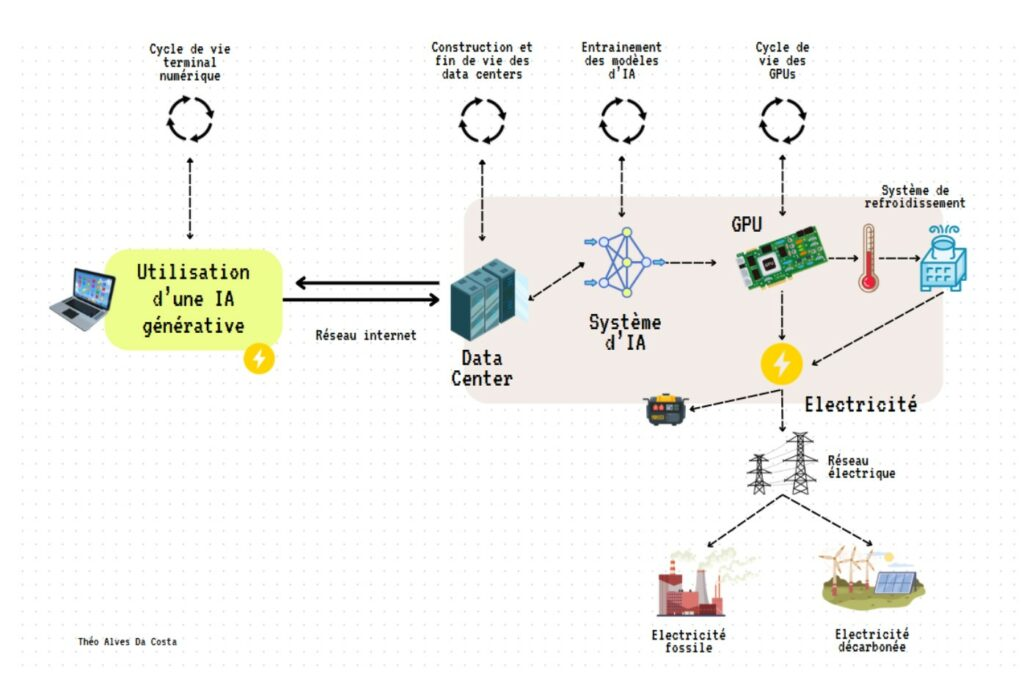
\includegraphics[width=\textwidth]{img/intro/IMAGE-6-credit-Bon-Pote-Theo-Alves-Da-costa-article-IA-1024x682.jpg}
  \end{center}

  {\footnotesize
  Ref : \href{https://bonpote.com/intelligence-artificielle-le-vrai-cout-environnemental-de-la-course-a-lia/}{\underline{Intelligence artificielle : le vrai coût environnemental de la course à l'IA}}}

\end{frame}

\begin{frame}{La donnée au centre !}
  \begin{center}
    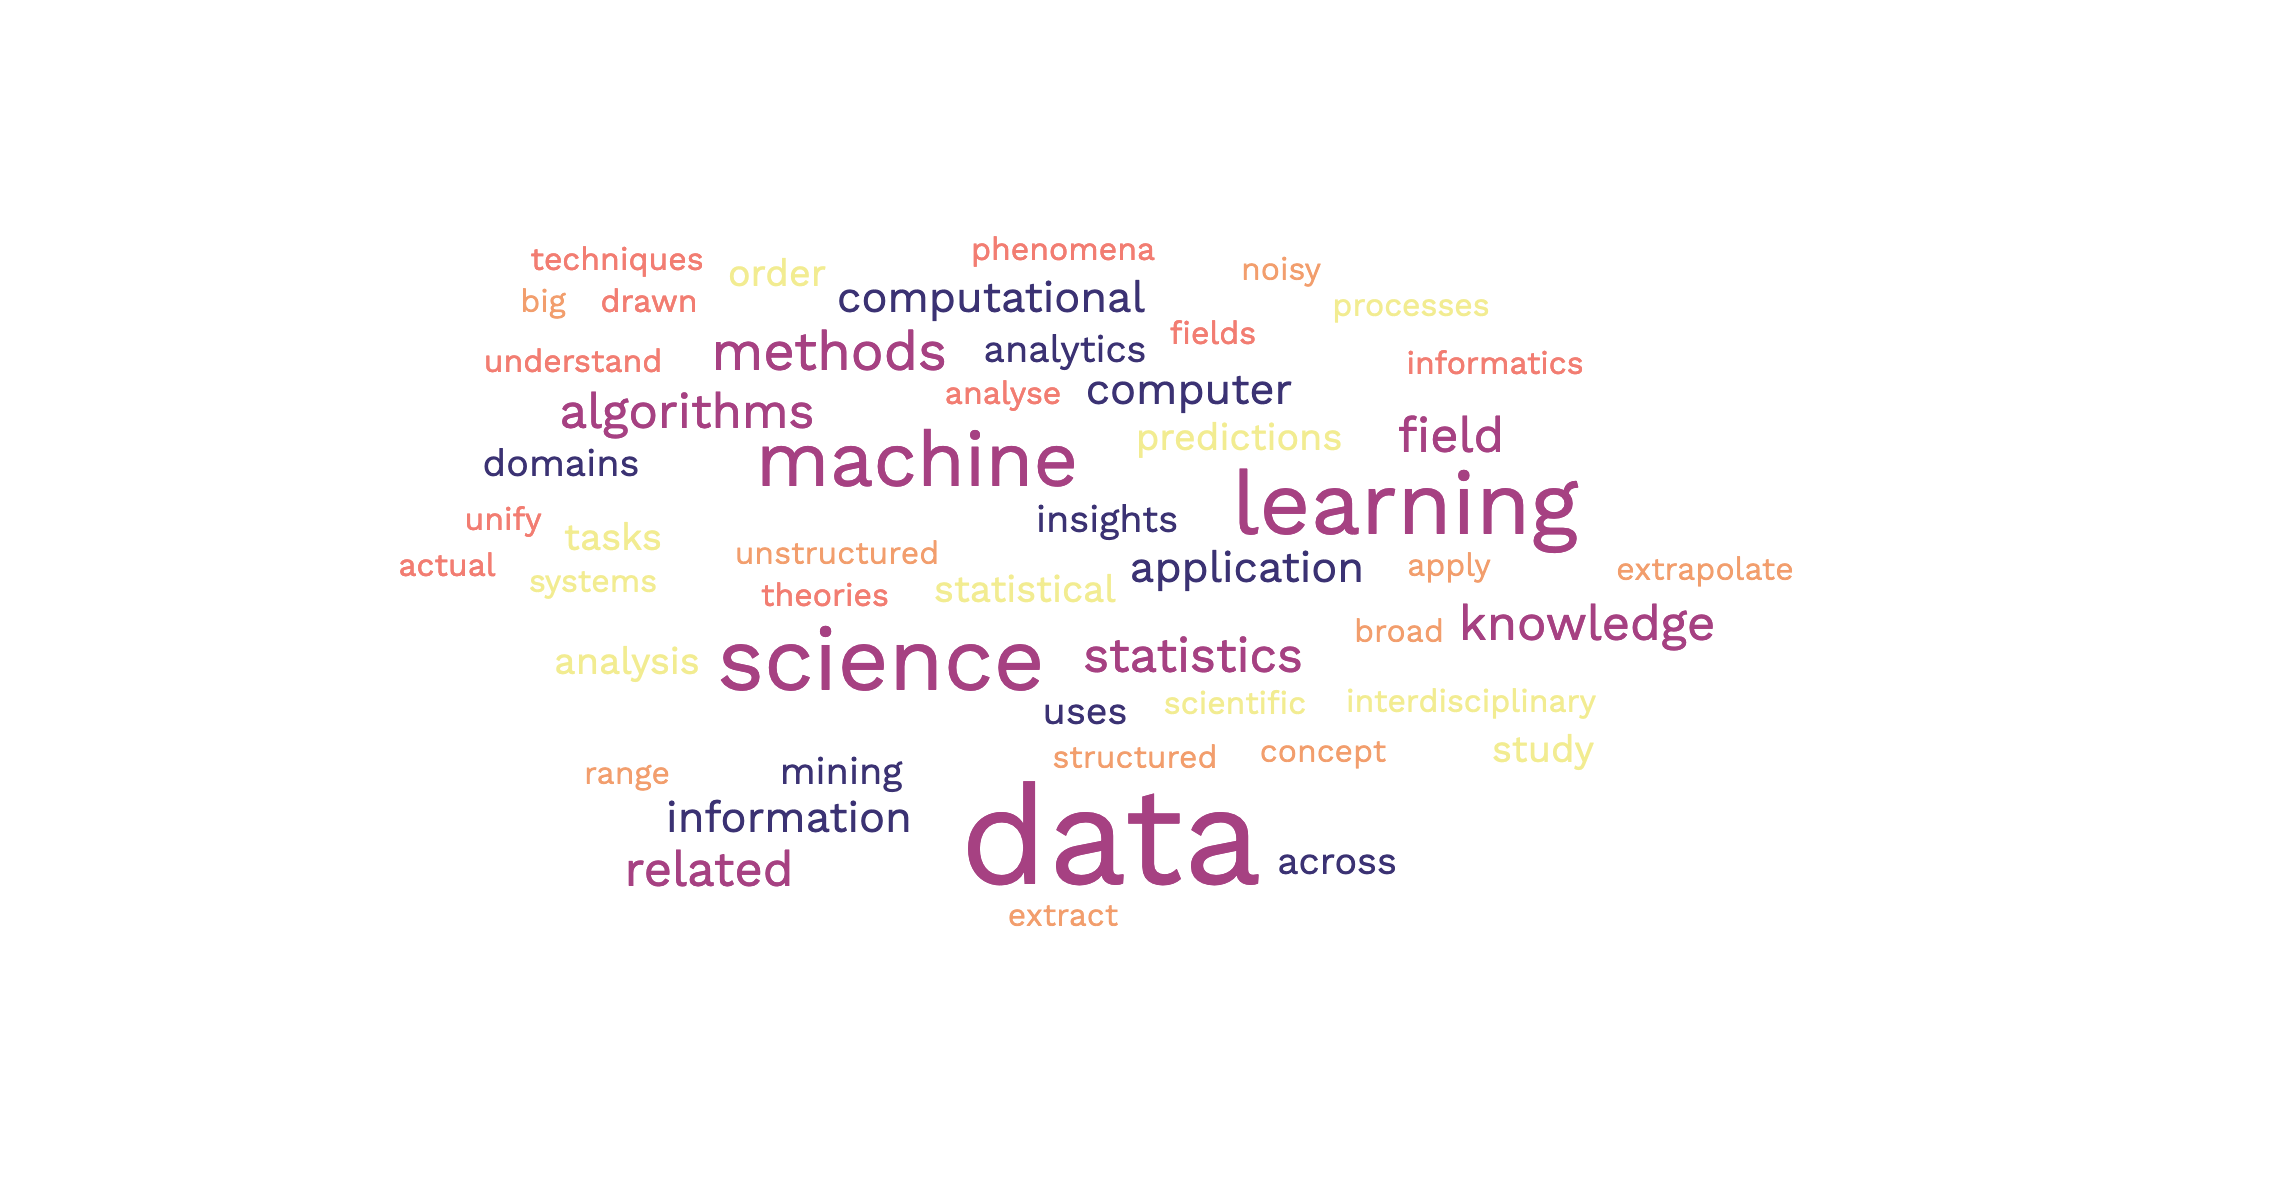
\includegraphics[width=\textwidth]{img/intro/word-cloud.png}
  \end{center}
\end{frame}

\begin{frame}{La donnée au centre !}
  \begin{center}
    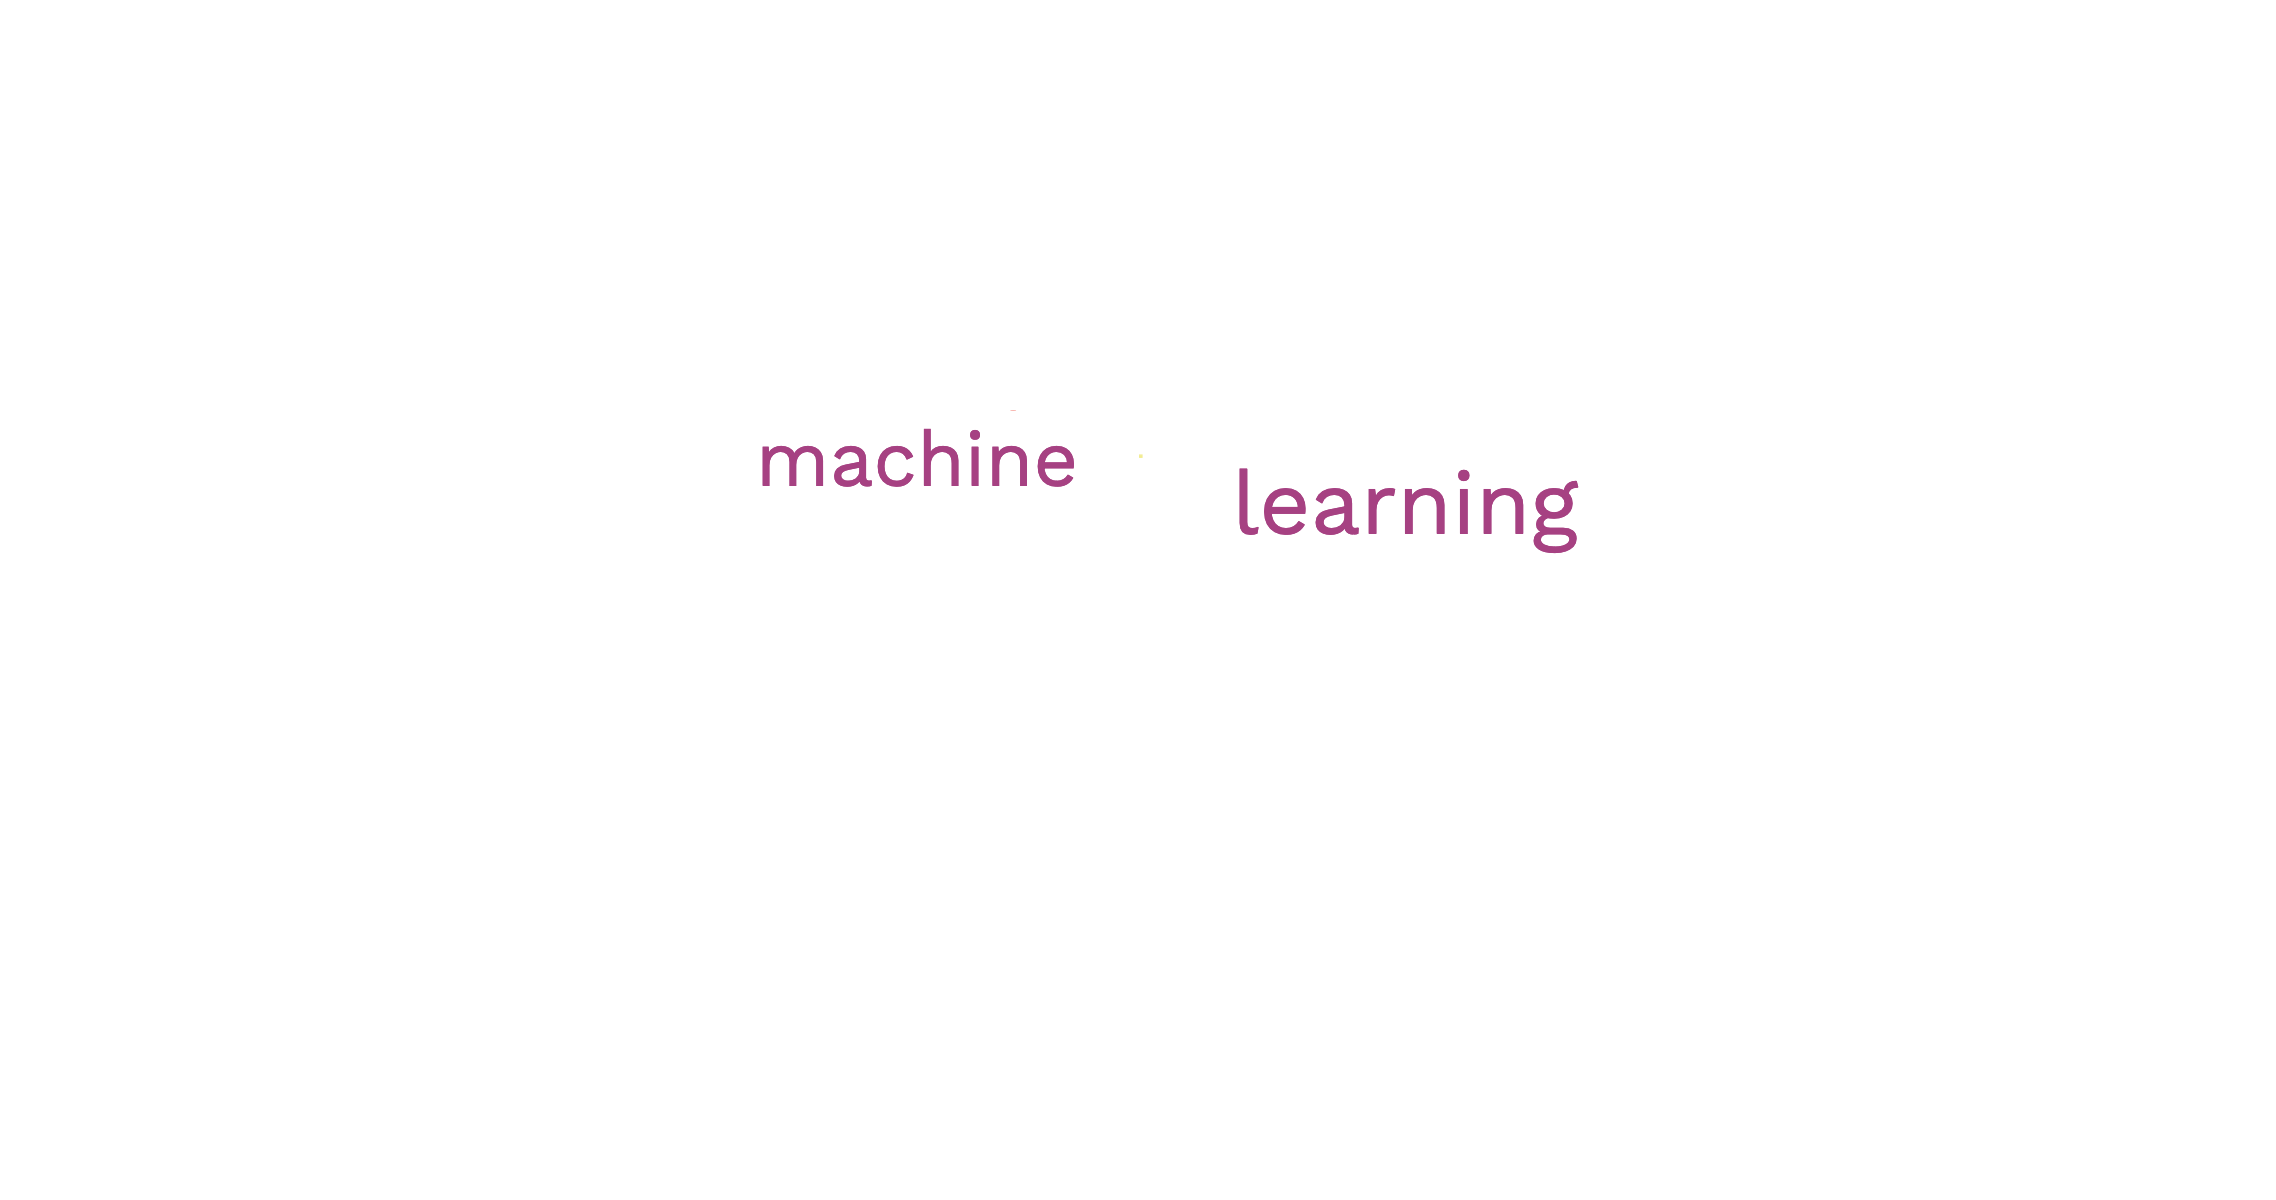
\includegraphics[width=\textwidth]{img/intro/word-cloud-2.png}
  \end{center}
\end{frame}



\section{Données}

\subsection{Data}

\begin{frame}{Qu'est-ce que la donnée ?}
    \begin{center}
        
\includegraphics[width=\textwidth]{img/ml/multimodal-1.png}
    \end{center}
\end{frame}

\begin{frame}{Qu'est-ce que la donnée ?}
    \begin{center}
        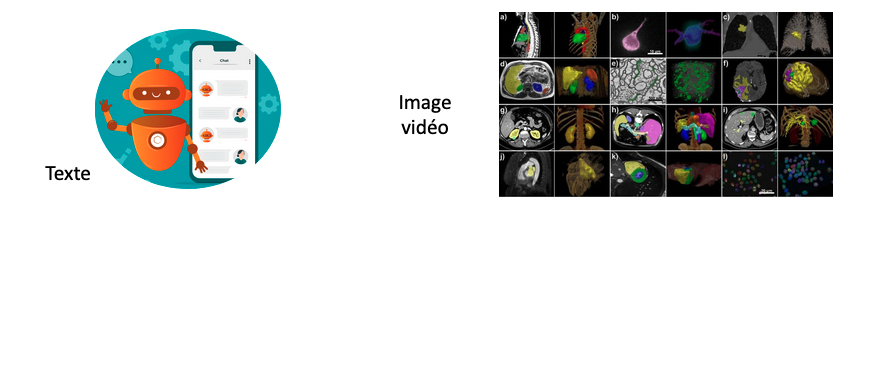
\includegraphics[width=\textwidth]{img/ml/multimodal-2.png}
    \end{center}
\end{frame}

\begin{frame}{Qu'est-ce que la donnée ?}
    \begin{center}
        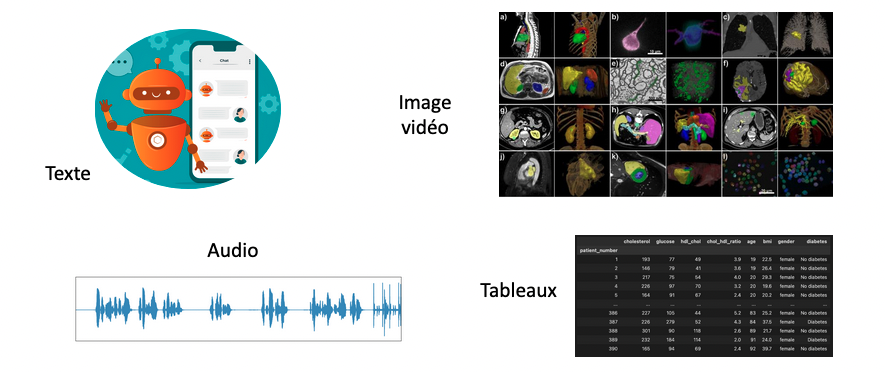
\includegraphics[width=\textwidth]{img/ml/multimodal-3.png}
    \end{center}
\end{frame}


\begin{frame}{Qu'est-ce que la donnée ?}

\textbf{Donnée} = de l'information que l'on peut enregistrer, stocker et analyser

\vspace{0.5cm}

La donnée peut être vue comme une \textbf{observation du monde} (social, physique, etc.).

\medskip

Exemples :
\begin{itemize}
    \item Produits : \textit{``Produit X, \$29.99, 1000 unités achetée en 2025''}
    \item Santé des patients : \textit{``Température 38°C, pression artérielle 120/80''}
    \item Une photo : \textit{``Ciel bleu, deux personnes, extérieur''}
\end{itemize}

\vspace{0.5cm}

\end{frame}

\begin{frame}{Trois types de données}

\begin{columns}[T]
\begin{column}{0.33\textwidth}
    \centering
    \textbf{Données tabulaires}\\
    \vspace{0.3cm}
    Structurées en lignes \& colonnes\\
    \vspace{0.2cm}
    \small Comme dans des tableurs
\end{column}

\begin{column}{0.33\textwidth}
    \centering
    \textbf{Images}\\
    \vspace{0.3cm}
    Information visuelle\\
    \vspace{0.2cm}
    \small Photos, dessins, scans
\end{column}

\begin{column}{0.33\textwidth}
    \centering
    \textbf{Données textuelles}\\
    \vspace{0.3cm}
    Langage naturel, écrit\\
    \vspace{0.2cm}
    \small Documents, emails, textes historiques
\end{column}
\end{columns}

\vspace{1cm}

\textbf{Chaque type de données correspond à des cas d'usage spécifiques}

\end{frame}



\begin{frame}
\frametitle{Type 1 : Données tabulaires}

\textbf{Qu'est-ce que c'est ?} L'information est organisée en un tableau
 
\vspace{0.5cm}

\textbf{Exemple: base de données clients}

\begin{table}
\small
\begin{tabular}{|l|c|c|c|}
\hline
\textbf{Name} & \textbf{Age} & \textbf{City} & \textbf{Purchase} \\
\hline
Alice & 32 & Paris & \$150 \\
Bob & 28 & Lyon & \$75 \\
Carol & 45 & Marseille & \$200 \\
\hline
\end{tabular}
\end{table}

\vspace{0.5cm}

\textbf{Chaque ligne} = une personne (ou produit, transaction, etc.)\\
\textbf{Chaque colonne} = une caractéristique

\vspace{0.3cm}

\textbf{Cas d'usage :} Predire le comportement client, recommender des produits

\end{frame}

\begin{frame}{Type 2 : image}

\textbf{Qu'est-ce que c'est ?} Photos, dessins, scans, screenshots

\vspace{0.5cm}

\begin{columns}
\begin{column}{0.5\textwidth}
    \textbf{Que voit un humain :}
    \begin{itemize}
        \item Un chat dans une combinaison spatiale
        \item Une bouteille dans un desert
    \end{itemize}
\end{column}

\begin{column}{0.5\textwidth}

  
\includegraphics[width=.5\textwidth]{img/intro/midjourney.png}

\end{column}
\end{columns}

\vspace{0.5cm}

\textbf{Cas d'usage :} Détection d'objets / forme, diagnostics médicaux

\end{frame}




\begin{frame}{Type 2 : image}

\textbf{Qu'est-ce que c'est ?} Photos, dessins, scans, screenshots

\vspace{0.5cm}

\begin{columns}
\begin{column}{0.5\textwidth}
    \textbf{Que voit un humain :}
    \begin{itemize}
        \item Un chat dans une combinaison spatiale
        \item Une bouteille dans un desert
    \end{itemize}
\end{column}

\begin{column}{0.5\textwidth}

  \textbf{Que voit un ordinateur :}
  \begin{itemize}
      \item Des millions de points (pixels)
      \item Chaque pixel correspond à une couleur spécifique
      \item Structure en grille RGB
  \end{itemize}
\end{column}
\end{columns}

\vspace{0.5cm}

\textbf{Cas d'usage :} Détection d'objets / forme, diagnostics médicaux

\end{frame}



\begin{frame}{Type 2 : image}

\textbf{Définition :} un tableau 3D, chaque pixel contenant une valeur numérique

\vspace{0.3cm}

\begin{center}
  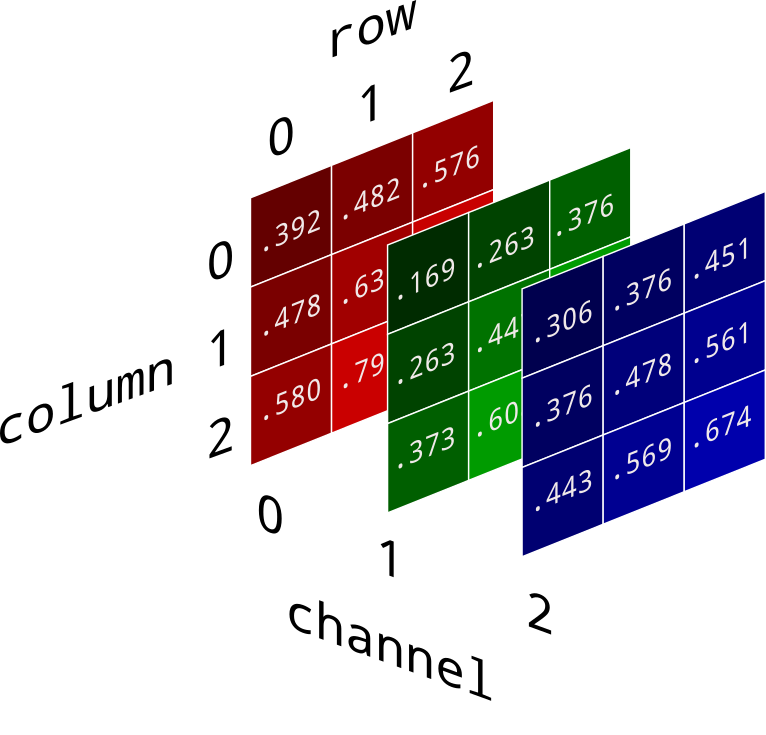
\includegraphics[width=.4\textwidth]{img/intro/rgb.png}
\end{center}

\vspace{0.3cm}

\textbf{Ordre de grandeurs :}
\begin{itemize}
  \item Image 224 x 224 pixels = 224 x 224 x 3 = 150 528 valeurs
  \item Photo 20M pixels = 5500 x 3700 x 3 = +60M valeurs
\end{itemize}

\end{frame}


\begin{frame}{Type 3 : données textuelles}

\textbf{Qu'est-ce que c'est ?} Contenu écrit, langage

\vspace{0.5cm}

\textbf{Exemples :}
\begin{itemize}
    \item Commentaires clients : \textit{``Super produit, envoi rapide !''}
    \item Réseaux sociaux, emails : \textit{``Just had the best coffee :-)''}
    \item Documents : contrats, raports, articles
\end{itemize}

\vspace{0.5cm}

\textbf{Challenge:} Le langage est ambigu, contextuel et créatif
\begin{itemize}
    \item ``banque'' = organisation financière ou médicale ?
    \item Sarcasme: ``Super, une autre réunion !''
\end{itemize}

\vspace{0.3cm}

\textbf{Cas d'usage :} Analyse de sentiments, traduction, chatbots

\end{frame}


\begin{frame}{Type 3 : données textuelles}

\textbf{Définition :} Séquences de symboles (caractères, mots, tokens)

\vspace{0.3cm}

\colorwarning{red}\textbf{Challenge :} les ordinateur traitent des nombres mais pas des mots

\vspace{0.3cm}

\textbf{Besoin de transformer les mots en nombres :}

\begin{enumerate}
    \item \textbf{Niveau ``caractère''} : chaque caractère remplacé par des nombres distincts
        \begin{itemize}
            \item[\textcolor{white}{x}] ``cat'' → [99, 97, 116]
        \end{itemize}
    
    \item \textbf{Niveau ``mot''} : encoder les mots (ou les sous-mot)
        \begin{itemize}
          \item[\textcolor{white}{x}] Word embeddings : chaque mot est un vector de nombres
          \item[\textcolor{white}{x}] → Nécessite la connaissance de l'ensemble des mots
        \end{itemize}
\end{enumerate}

\end{frame}




\begin{frame}{Trois types de données : approches différentes}

Différents type de données nécessitent \textbf{différentes approches IA}:

\vspace{0.5cm}

\begin{tabular}{l|l|l}
\textbf{Type} & \textbf{Approche} & \textbf{Dimensionnalité}\\
\hline
Tabulaire & Modèles statistiques & \textcolor{blue}{Modérée}\\
          & arbres de décision   & 10-1000 variables \\
Image & Vision par ordinateur    & \textcolor{red}{Très grande}\\
      & réseaux de neurones      & 100k-70M valeurs\\
Texte & Traitement automatique   & \textcolor{orange}{Grande}\\
      & du langage (NLP)         & 50k-100k mots\\
\end{tabular}

\onslide<2>
\colorwarning{orange}Les LLMs sont construits sur des \textcolor{red}{tokens} et pas uniquement sur des mots. La dimensionnalité peut atteindre des trillions !

\end{frame}

\begin{frame}{Trois types de données : approches différentes}

    \onslide<1->

      \textbf{Modèle tabulaire}
      \bigskip

      \begin{center}
        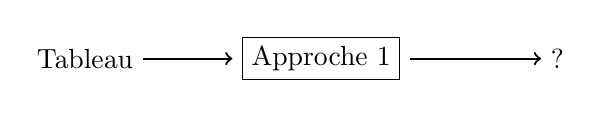
\begin{tikzpicture}[
          every node/.style={align=center},
          arrow/.style={->, thick}
        ]
          \node (table) at (-3,0) {Tableau};
          
          % Box in the middle
          \node (box) at (0,0) {\boxed{\mbox{Approche 1}}};
          
          % Text on the right
          \node (right) at (3,0) {?};
          
          % Arrows
          \draw[arrow] (table) -- (box);
          \draw[arrow] (box) -- (right);
        \end{tikzpicture}
      \end{center}

    \onslide<2->
      \textbf{Modèle de vision par ordinateur}
      \bigskip

      \begin{center}
        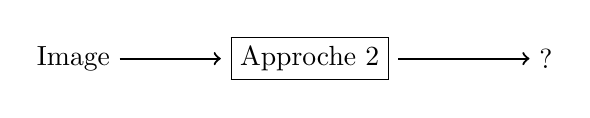
\begin{tikzpicture}[
          every node/.style={align=center},
          arrow/.style={->, thick}
        ]
          \node (image) at (-3,0) {Image};
          
          % Box in the middle
          \node (box) at (0,0) {\boxed{\mbox{Approche 2}}};
          
          % Text on the right
          \node (right) at (3,0) {?};
          
          % Arrows
          \draw[arrow] (image) -- (box);
          \draw[arrow] (box) -- (right);
        \end{tikzpicture}
      \end{center}
    \onslide<3>
      \textbf{Modèle de NLP}
      \bigskip
      
      \begin{center}
        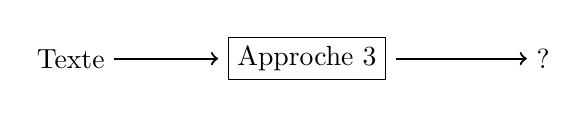
\begin{tikzpicture}[
          every node/.style={align=center},
          arrow/.style={->, thick}
        ]
          \node (text) at (-3,0) {Texte};
          
          % Box in the middle
          \node (box) at (0,0) {\boxed{\mbox{Approche 3}}};
          
          % Text on the right
          \node (right) at (3,0) {?};
          
          % Arrows
          \draw[arrow] (text) -- (box);
          \draw[arrow] (box) -- (right);
        \end{tikzpicture}
      \end{center}

\end{frame}

\begin{frame}{Trois types de données : approches différentes}

      \textbf{Modèle \textcolor{red}{multimodal}}
      \bigskip
      
      \begin{center}
        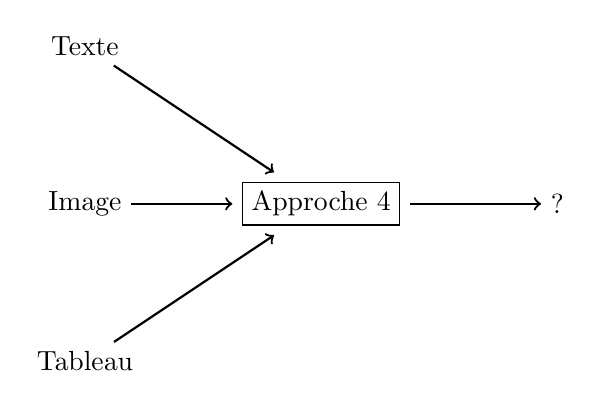
\begin{tikzpicture}[
          every node/.style={align=center},
          arrow/.style={->, thick}
        ]
          \node (text) at (-3,-2) {Tableau};
          \node (image) at (-3,0) {Image};
          \node (table) at (-3,2) {Texte};
          
          % Box in the middle
          \node (box) at (0,0) {\boxed{\mbox{Approche 4}}};
          
          % Text on the right
          \node (right) at (3,0) {?};
          
          % Arrows
          \draw[arrow] (table) -- (box);
          \draw[arrow] (image) -- (box);
          \draw[arrow] (text) -- (box);
          \draw[arrow] (box) -- (right);
        \end{tikzpicture}
      \end{center}
  
\end{frame}


\section{Fouille de Données}

\begin{frame}
\frametitle{Introduction à la Fouille de Données}
\framesubtitle{Data Mining}

\textbf{Définition}

\vspace{0.3cm}

La fouille de données est le processus d'\textbf{extraction de connaissances} implicites, utiles et compréhensibles à partir de grandes quantités de données.

\vspace{0.3cm}

\textbf{Elle combine :}
\begin{itemize}
    \item Statistiques
    \item Intelligence artificielle (apprentissage automatique)
    \item Visualisation
    \item Algorithmes de recherche de motifs
\end{itemize}

\end{frame}

\begin{frame}{Historique du Data Mining}

\begin{itemize}
    \item<+-> \textbf{Années 1960-1970}
        \begin{itemize}
            \item Développement des bases de données relationnelles (SQL)
            \item Premières techniques d'analyse statistique
        \end{itemize}

    \vspace{0.2cm}
    \item<+-> \textbf{Années 1980-1990}
        \begin{itemize}
            \item Boom avec l'augmentation des volumes de données
            \item Augmentation de la puissance de calcul
            \item Apparition du terme "data mining" dans les années 1990
            \item Popularisé par le projet KDD (Knowledge Discovery in Databases)
        \end{itemize}

    \vspace{0.2cm}
    \item<+-> \textbf{Années 2000 à aujourd'hui}
        \begin{itemize}
            \item Intégration avec l'IA et le big data
            \item Démocratisation : outils accessibles (Python, R, Tableau)
        \end{itemize}
\end{itemize}

\end{frame}

\begin{frame}{Applications : Finance}

\textbf{Problème :} Détection de fraudes dans les transactions bancaires

\vspace{0.3cm}

\textbf{Solution :}
\begin{itemize}
    \item<+-> Clustering pour identifier les comportements inhabituels
        \begin{itemize}
            \item Exemple : dépenses soudaines anormales
        \end{itemize}
    \item<+-> Modèles de classification pour prédire si une transaction est frauduleuse
\end{itemize}

\vspace{0.3cm}

\onslide<2>
\textbf{Algorithmes utilisés :}
\begin{itemize}
    \item Arbres de décision
    \item Réseaux de neurones
\end{itemize}

\end{frame}

\begin{frame}{Applications : Santé}

\textbf{Problème :} Prédiction des risques de maladies chroniques

\vspace{0.3cm}

\textbf{Solution :}
\begin{itemize}
    \item<+-> Analyse de dossiers médicaux
        \begin{itemize}
            \item Identifier des corrélations entre symptômes et diagnostics
        \end{itemize}
    \item<+-> Visualisation des résultats pour aider les médecins
        \begin{itemize}
            \item Exemple : heatmaps des zones à risque dans une population
        \end{itemize}
\end{itemize}

\end{frame}

\begin{frame}{Applications : Marketing}

\textbf{Problème :} Segmentation des clients pour personnaliser les offres

\vspace{0.3cm}

\textbf{Solution :}
\begin{itemize}
    \item<+-> \textbf{Clustering (k-means)}
        \begin{itemize}
            \item Regrouper les clients selon leurs comportements d'achat
        \end{itemize}

    \vspace{0.2cm}
    \item<+-> \textbf{Règles d'association}
        \begin{itemize}
            \item Identifier des produits souvent achetés ensemble
        \end{itemize}
\end{itemize}

\end{frame}

\begin{frame}{Applications : Retail et Industrie}

\begin{columns}
\begin{column}{0.48\textwidth}
    \colormark{blue}\textbf{Retail :}
    \begin{itemize}
        \item \textbf{Problème :} Optimisation des stocks et prévision des ventes
        \item \textbf{Solution :}
        \begin{itemize}
            \item Séries temporelles pour prédire la demande
            \item Analyse de paniers d'achat
        \end{itemize}
    \end{itemize}
\end{column}

\begin{column}{0.48\textwidth}
    \onslide<2>
    \colormark{blue}\textbf{Industrie :}
    \begin{itemize}
        \item \textbf{Problème :} Maintenance prédictive des machines
        \item \textbf{Solution :}
        \begin{itemize}
            \item Analyse des données de capteurs
            \item Réduction de dimensionnalité (PCA)
        \end{itemize}
    \end{itemize}
\end{column}
\end{columns}

\end{frame}

\begin{frame}{Méthodologie : CRISP-DM}
\framesubtitle{Cross-Industry Standard Process for Data Mining}

\textbf{Une approche structurée en 6 étapes :}

\vspace{0.3cm}

\begin{enumerate}
    \item Compréhension du problème métier
    \item Compréhension des données
    \item Préparation des données
    \item Modélisation
    \item Évaluation
    \item Déploiement et maintenance
\end{enumerate}

\end{frame}

\begin{frame}{CRISP-DM : 1. Compréhension du problème}

\textbf{Objectif :} Définir clairement le problème à résoudre

\vspace{0.3cm}

\begin{itemize}
    \item Exemple : "Comment réduire le taux d'attrition des clients ?"
    \item Impliquer les parties prenantes
    \item Définir un objectif clair et actionnable
\end{itemize}

\vspace{0.5cm}

\onslide<2>
\textbf{Importance de la formulation de la question :}

\vspace{0.2cm}

\begin{itemize}
    \item \textcolor{red}{Mauvaise question :} "Quelles sont les tendances de nos ventes ?"
        \begin{itemize}
            \item Trop vague, difficile à actionner
        \end{itemize}
    \item \textcolor{green}{Bonne question :} "Quels produits ont un taux de retour élevé et quels facteurs (taille, couleur, saison) y contribuent ?"
        \begin{itemize}
            \item Permet d'identifier des leviers d'amélioration
        \end{itemize}
\end{itemize}

\end{frame}

\begin{frame}{CRISP-DM : 2. Compréhension des données}

\textbf{Exploration (EDA) :}

\vspace{0.3cm}

\begin{itemize}
    \item<+-> Analyser la distribution des données
    \item<+-> Identifier les valeurs manquantes ou aberrantes
    \item<+-> Visualisation : graphiques
        \begin{itemize}
            \item Histogrammes
            \item Boxplots
            \item Heatmaps
        \end{itemize}
\end{itemize}

\end{frame}

\begin{frame}{CRISP-DM : 3. Préparation des données}

\textbf{Nettoyage :}

\vspace{0.3cm}

\begin{itemize}
    \item<+-> Gestion des valeurs manquantes
        \begin{itemize}
            \item Imputation
            \item Suppression
        \end{itemize}

    \vspace{0.2cm}
    \item<+-> Normalisation
        \begin{itemize}
            \item Mise à l'échelle pour algorithmes (ex : k-means)
        \end{itemize}
\end{itemize}

\vspace{0.3cm}

\onslide<2>
\textbf{Transformation :}
\begin{itemize}
    \item Création de nouvelles variables
    \item Exemples : ratio, catégories
\end{itemize}

\end{frame}

\begin{frame}{CRISP-DM : 4. Modélisation}

\textbf{Choix du modèle en fonction du problème :}

\vspace{0.3cm}

\begin{itemize}
    \item<+-> \textbf{Classification} : prédire une catégorie
        \begin{itemize}
            \item Exemple : spam/non-spam
            \item Algorithmes : Arbres de décision, SVM, Réseaux de neurones
        \end{itemize}

    \vspace{0.2cm}
    \item<+-> \textbf{Régression} : prédire une valeur continue
        \begin{itemize}
            \item Exemple : prix d'une maison
        \end{itemize}

    \vspace{0.2cm}
    \item<+-> \textbf{Clustering} : regrouper des données sans étiquettes
        \begin{itemize}
            \item Exemple : segmentation client
        \end{itemize}

    \vspace{0.2cm}
    \item<+-> \textbf{Règles d'association} : trouver des motifs
        \begin{itemize}
            \item Exemple : "30\% des clients qui achètent X achètent aussi Y"
        \end{itemize}
\end{itemize}

\end{frame}

\begin{frame}{CRISP-DM : 5. Évaluation}

\textbf{Métriques adaptées :}

\vspace{0.3cm}

\begin{itemize}
    \item<+-> \textbf{Classification :}
        \begin{itemize}
            \item Précision
            \item Rappel
            \item F1-score
        \end{itemize}

    \vspace{0.2cm}
    \item<+-> \textbf{Régression :}
        \begin{itemize}
            \item RMSE (Root Mean Squared Error)
        \end{itemize}
\end{itemize}

\vspace{0.3cm}

\onslide<2>
\textbf{Validation croisée :}
\begin{itemize}
    \item Pour éviter le surfitement (overfitting)
\end{itemize}

\end{frame}

\begin{frame}{CRISP-DM : 6. Déploiement}

\textbf{Déploiement et maintenance :}

\vspace{0.3cm}

\begin{itemize}
    \item<+-> Intégration du modèle dans un système opérationnel
    \item<+-> Surveillance continue
        \begin{itemize}
            \item Détecter la dérive des données
            \item Détecter la perte de performance
        \end{itemize}
\end{itemize}

\end{frame}

\begin{frame}{Limites : Problèmes courants}

\begin{enumerate}
    \item<+-> \textbf{Mauvaise formulation de la question}
        \begin{itemize}
            \item Risque : résultats inutiles ou non actionnables
            \item Solution : Co-construction avec les métiers
        \end{itemize}

    \vspace{0.2cm}
    \item<+-> \textbf{Données insuffisantes ou de mauvaise qualité}
        \begin{itemize}
            \item Problème du "rare event" : cas rares nécessitent beaucoup de données
            \item Biais dans les données
            \item Exemple : modèle de recrutement biaisé
        \end{itemize}

    \vspace{0.2cm}
    \item<+-> \textbf{Surfitement (overfitting)}
        \begin{itemize}
            \item Le modèle mémorise mais ne généralise pas
            \item Solution : validation croisée, régularisation
        \end{itemize}
\end{enumerate}

\end{frame}

\begin{frame}{Limites : Interprétabilité}

\textbf{Problème :}

\vspace{0.3cm}

\begin{itemize}
    \item Certains algorithmes sont des "boîtes noires"
    \item Exemple : réseaux de neurones profonds
\end{itemize}

\vspace{0.5cm}

\onslide<2>
\textbf{Solution :}
\begin{itemize}
    \item Privilégier des modèles explicables quand c'est possible
    \item Arbres de décision
    \item Régression linéaire
\end{itemize}

\end{frame}

\begin{frame}{Bonnes pratiques}

\small
\begin{tabular}{|p{3.5cm}|p{3cm}|p{3cm}|}
\hline
\textbf{Bonne pratique} & \textbf{Description} & \textbf{Exemple} \\
\hline
Question claire et actionnable & Impliquer les parties prenantes & "Réduire coûts logistiques de 10\% sans impacter satisfaction" \\
\hline
Qualité des données & Nettoyer et valider avant analyse & Supprimer doublons, imputer valeurs manquantes \\
\hline
Validation robuste & Cross-validation pour généralisation & Diviser données en 5 folds \\
\hline
Documentation & Documenter chaque étape & Notebooks Jupyter commentés \\
\hline
Éthique et transparence & Auditer pour éviter biais & Vérifier non-discrimination \\
\hline
\end{tabular}

\end{frame}

\begin{frame}{Collecte de données : Sources}

\textbf{1. Données structurées}
\begin{itemize}
    \item Bases de données relationnelles (SQL)
    \item Fichiers CSV/Excel
    \item Exemple : bases clients, transactions
\end{itemize}

\vspace{0.3cm}

\onslide<2->
\textbf{2. Données non structurées}
\begin{itemize}
    \item Textes (emails, avis clients)
    \item Images, vidéos
    \item Exemple : analyse de sentiments (text mining)
\end{itemize}

\vspace{0.3cm}

\onslide<3>
\textbf{3. Données externes}
\begin{itemize}
    \item Open data (INSEE, Eurostat)
    \item APIs (météo, trafic)
    \item Web scraping (respecter RGPD)
\end{itemize}

\end{frame}

\begin{frame}{Collecte de données : Défis}

\textbf{Accès et légalité :}
\begin{itemize}
    \item Respecter les réglementations (RGPD)
    \item Obtenir les droits d'utilisation
\end{itemize}

\vspace{0.3cm}

\onslide<2->
\textbf{Nettoyage et préparation :}
\begin{itemize}
    \item Données bruitées, incohérentes, manquantes
    \item Techniques : imputation, suppression des doublons, normalisation
\end{itemize}

\vspace{0.3cm}

\onslide<3>
\textbf{Intégration :}
\begin{itemize}
    \item Fusionner des données de sources différentes
    \item Exemple : données internes + données marché
\end{itemize}

\end{frame}

\begin{frame}{Algorithmes spécifiques au data mining}

\begin{enumerate}
    \item<+-> \textbf{Règles d'association}
        \begin{itemize}
            \item Découvrir des associations entre variables
            \item Exemple : catégorie socio-professionnelle vs certains produits
            \item Utilisé en marketing pour recommandations
        \end{itemize}

    \vspace{0.3cm}
    \item<+-> \textbf{Détection d'anomalies}
        \begin{itemize}
            \item Identifier des observations rares ou suspectes
            \item Exemple : fraudes bancaires
            \item Techniques : isolation forest, auto-encoders
        \end{itemize}
\end{enumerate}

\end{frame}

\begin{frame}{Cas pratique : Optimisation supermarché}
\framesubtitle{Réduire le gaspillage et optimiser les promotions}

\textbf{Scénario :}

\vspace{0.2cm}

Vous travaillez pour un supermarché qui souhaite :
\begin{itemize}
    \item Optimiser ses promotions
    \item Réduire le gaspillage alimentaire
\end{itemize}

\vspace{0.3cm}

\textbf{Comment aborderiez-vous ce problème ?}

\end{frame}

\begin{frame}{Cas pratique : 1. Formulation de la question}

\textbf{Questions à poser :}

\vspace{0.3cm}

\begin{itemize}
    \item "Quels produits ont un taux de retour élevé (gaspillage) ?"
    \item "Quels facteurs y contribuent ?"
        \begin{itemize}
            \item Prix
            \item Saison
            \item Emplacement en rayon
        \end{itemize}
    \item "Quelles promotions croisées maximisent les ventes ?"
        \begin{itemize}
            \item Exemple : fromage + vin
            \item Sans impacter la marge
        \end{itemize}
\end{itemize}

\end{frame}

\begin{frame}{Cas pratique : 2-3. Collecte et Préparation}

\textbf{Collecte des données :}
\begin{itemize}
    \item Données internes : ventes, stocks, promotions passées
    \item Données externes : météo, événements locaux
\end{itemize}

\vspace{0.3cm}

\onslide<2>
\textbf{Préparation :}
\begin{itemize}
    \item Nettoyage : supprimer transactions incomplètes
    \item Imputer valeurs manquantes
    \item Créer nouvelles variables :
        \begin{itemize}
            \item Ratio gaspillage = (stock final - ventes) / stock initial
        \end{itemize}
\end{itemize}

\end{frame}

\begin{frame}{Cas pratique : 4. Modélisation}

\textbf{Pour le gaspillage :}
\begin{itemize}
    \item<+-> Régression pour prédire le taux de gaspillage
        \begin{itemize}
            \item En fonction du prix et de la saison
        \end{itemize}
    \item<+-> Clustering pour segmenter les produits
        \begin{itemize}
            \item Selon sensibilité au gaspillage
        \end{itemize}
\end{itemize}

\vspace{0.3cm}

\onslide<3>
\textbf{Pour les promotions croisées :}
\begin{itemize}
    \item Règles d'association
        \begin{itemize}
            \item Trouver produits souvent achetés ensemble
        \end{itemize}
\end{itemize}

\end{frame}

\begin{frame}{Cas pratique : 5-6. Évaluation et Déploiement}

\textbf{Évaluation :}
\begin{itemize}
    \item Pour la régression : RMSE pour mesurer l'erreur
    \item Pour les règles d'association : support, confidence, lift
\end{itemize}

\vspace{0.3cm}

\onslide<2>
\textbf{Déploiement :}
\begin{itemize}
    \item Recommander promotions ciblées
        \begin{itemize}
            \item "Achetez le fromage et obtenez 20\% sur le vin"
        \end{itemize}
    \item Mettre en place un tableau de bord
        \begin{itemize}
            \item Suivre l'impact des promotions
        \end{itemize}
\end{itemize}

\end{frame}

\begin{frame}{Outils et ressources}

\textbf{Pour la visualisation :}
\begin{itemize}
    \item Tableau, Power BI (drag-and-drop)
    \item Idéal pour les non-techniciens
\end{itemize}

\vspace{0.3cm}

\onslide<2->
\textbf{Pour le nettoyage et l'analyse :}
\begin{itemize}
    \item Excel (formules avancées, Power Query)
    \item Python : Pandas, Matplotlib/Seaborn, Scikit-learn
    \item R : analyses statistiques avancées
\end{itemize}

\end{frame}

\begin{frame}{Conclusion : Points clés}

\textbf{Bonnes pratiques à retenir :}

\vspace{0.3cm}

\begin{enumerate}
    \item \textbf{Poser la bonne question}

    Impliquer les métiers, objectif clair et actionnable

    \item \textbf{Travailler avec des données de qualité}
    
    Nettoyage rigoureux, gestion des valeurs manquantes

    \item \textbf{Évaluer correctement les modèles}
    
    Validation croisée, métriques adaptées

    \item \textbf{Documenter et expliquer}
    
    Modèle compréhensible par tous

    \item \textbf{Penser à l'éthique}
    
    Auditer les données pour éviter les biais

\end{enumerate}

\end{frame}

\begin{frame}{Message final}

\textbf{Le data mining n'est pas une magie}

\vspace{0.3cm}

C'est un processus structuré qui repose sur :

\vspace{0.3cm}

\begin{itemize}
    \item Une \textcolor{blue}{bonne formulation du problème}
    \item Des \textcolor{blue}{données propres et représentatives}
    \item Des \textcolor{blue}{méthodes adaptées}
    \item Et une \textcolor{blue}{évaluation rigoureuse}
\end{itemize}

\vspace{0.5cm}

En suivant ces bonnes pratiques, même sans expertise technique avancée, il est possible de tirer des insights puissants pour innover et prendre des décisions éclairées.

\end{frame}


\section{Analyses statistiques et \\visualisation de données}



\begin{frame}{Analyse statistique}

  \begin{block}{Analyse statistique}
    \medskip
      \begin{itemize}
        \item<+-> Tirer de l'information des données dans l'objectif de \textbf{prendre des décisions}
        \item<+-> Identifier les tendances et les relations entre les différentes variables
        \item<+-> Statistiques : des méthodes mathématiques utilisées pour collecter, analyser et interpréter des données
        \item<+-> Les statistiques incluent la probabilité théorique, l'estimation des moyennes et des médianes, les tests de hypothèses, etc.
      \end{itemize}
  \end{block}
\end{frame}

\begin{frame}{Analyse statistique}
  \begin{block}{Objectifs}
    \medskip
    \begin{itemize}
      \item<+-> Tirer des insights des données pour prendre des décisions
      \item<+-> Identifier tendances et relations entre variables
    \end{itemize}
  \end{block}

  \onslide<3->{
    \begin{block}{Définition}
      \medskip
      \begin{itemize}
        \item<3-> Méthodes mathématiques pour collecter, analyser et interpréter des données
        \item<4-> Deux branches principales :
        \begin{enumerate}
          \item \textbf{Descriptive} : décrire les données (moyennes, graphiques)
          \item \textbf{Inférentielle} : généraliser à partir d'un échantillon
        \end{enumerate}
      \end{itemize}
    \end{block}
  }

  \onslide<5->{
    \begin{exampleblock}{Exemple concret}
      \medskip
      Un supermarché utilise la moyenne des ventes pour ajuster ses stocks
    \end{exampleblock}
  }
\end{frame}

\begin{frame}{Concepts statistiques essentiels}
  \begin{enumerate}
    \item<+-> \textbf{Mesures de tendance centrale :}
    \begin{itemize}
      \item Moyenne (sensible aux extrêmes)
      \item Médiane (robuste aux extrêmes)
    \end{itemize}

    \item<+-> \textbf{Mesures de dispersion :}
    \begin{itemize}
      \item Écart-type : variabilité autour de la moyenne
      \item Intervalle interquartile (IQR) : moins sensible aux extrêmes
    \end{itemize}

    \item<+-> \textbf{Corrélation vs causalité :}
    \begin{itemize}
      \item Exemple : ``Plus il y a de glaces vendues, plus il y a de noyades'' \\ $\Rightarrow$ corrélation $\neq$ causalité !
    \end{itemize}

    \item<+-> \textbf{Tests d'hypothèses :}
    \begin{itemize}
      \item Tester si un résultat est significatif (ex : un nouveau médicament est-il efficace ?)
    \end{itemize}
  \end{enumerate}
\end{frame}

\begin{frame}{Applications industrielles}
  \begin{block}{Domaines d'application}
    \medskip
    \begin{itemize}
      \item<+-> \textbf{Marketing} : segmentation client, A/B testing
      \item<+-> \textbf{Finance} : modélisation des risques, détection de fraudes
      \item<+-> \textbf{Santé} : études cliniques, analyse de données médicales
    \end{itemize}
  \end{block}

  \onslide<4->{
    \begin{alertblock}{Pièges à éviter}
      \medskip
      \begin{enumerate}
        \item Biais dans les données (échantillon non représentatif)
        \item Surinterprétation (corrélation $\neq$ causalité)
        \item Données de mauvaise qualité (manquantes, bruitées)
      \end{enumerate}
    \end{alertblock}
  }

  \onslide<5->{
    \begin{block}{Bonnes pratiques}
      \medskip
      \begin{itemize}
        \item Vérifier la qualité des données avant analyse
        \item Choisir les bonnes métriques (moyenne vs médiane)
        \item Documenter et itérer sur les modèles
      \end{itemize}
    \end{block}
  }
\end{frame}

\begin{frame}{Outils pour l'analyse statistique}
  \begin{block}{Outils disponibles}
    \medskip
    \begin{itemize}
      \item<+-> \textbf{Excel/Google Sheets} : fonctions de base, graphiques
      \item<+-> \textbf{Python/R} : Pandas, Scikit-learn, Statsmodels
      \item<+-> \textbf{Tableau/Power BI} : visualisation interactive
    \end{itemize}
  \end{block}

  \onslide<4->{
    \begin{exampleblock}{Exemple concret : Analyse des ventes}
      \medskip
      \begin{enumerate}
        \item Données : ventes mensuelles + prix/promotions/saison
        \item Analyse descriptive : moyennes, graphiques temporels
        \item Modélisation : régression linéaire pour prédire les ventes
        \item Résultats actionnables : ``Les promotions augmentent les ventes de 15\%''
      \end{enumerate}
    \end{exampleblock}
  }
\end{frame}

\begin{frame}{Visualisation de données}

\end{frame}


\begin{frame}{Visualisation de données}
  \begin{block}{Visualisation}
    \medskip
    ``La visualisation est un processus \textcolor{blue}{cognitif} qui permet de former une \textcolor{blue}{image mentale} pour découvrir, expliquer et \textcolor{red}{prendre des décisions}.''
  \end{block}

  \onslide<2>{
    \begin{block}{Visualisation de données}
      \medskip
      ``La visualisation de données est la représentation visuelle informatisée de données \textcolor{blue}{pour amplifier} la cognition.''
    \end{block}
    
    \bigskip
    Source : \href{https://maelfabien.github.io/machinelearning/Dataviz/}{\underline{maelfabien.github.io}}
  }
\end{frame}

\begin{frame}{Intérêt de la visualisation de données}
  \centering
  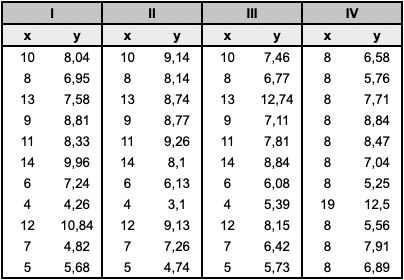
\includegraphics[scale=.5]{img/intro/anscombe.png}

  Anscombe's quartet
\end{frame}

\begin{frame}{Intérêt de la visualisation de données}
  \begin{center}
    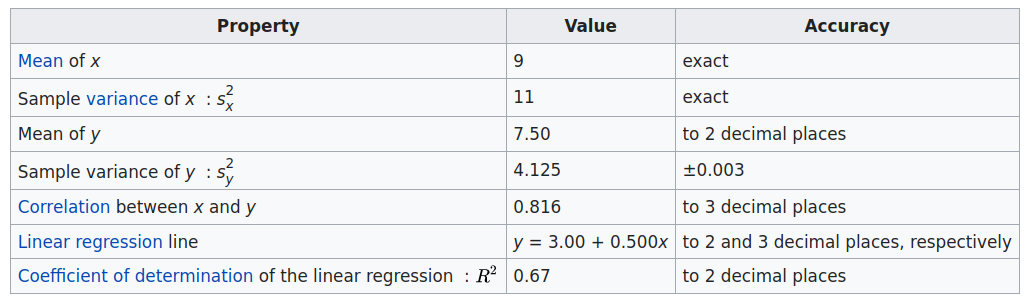
\includegraphics[width=\textwidth]{img/intro/anscombe_wikipedia.png}
    
    Anscombe's quartet
  \end{center}

  \bigskip
  \bigskip
  \bigskip
  \bigskip
  \footnotesize
  Source : Wikipedia
\end{frame}

\begin{frame}{Intérêt de la visualisation de données}
  \begin{center}
    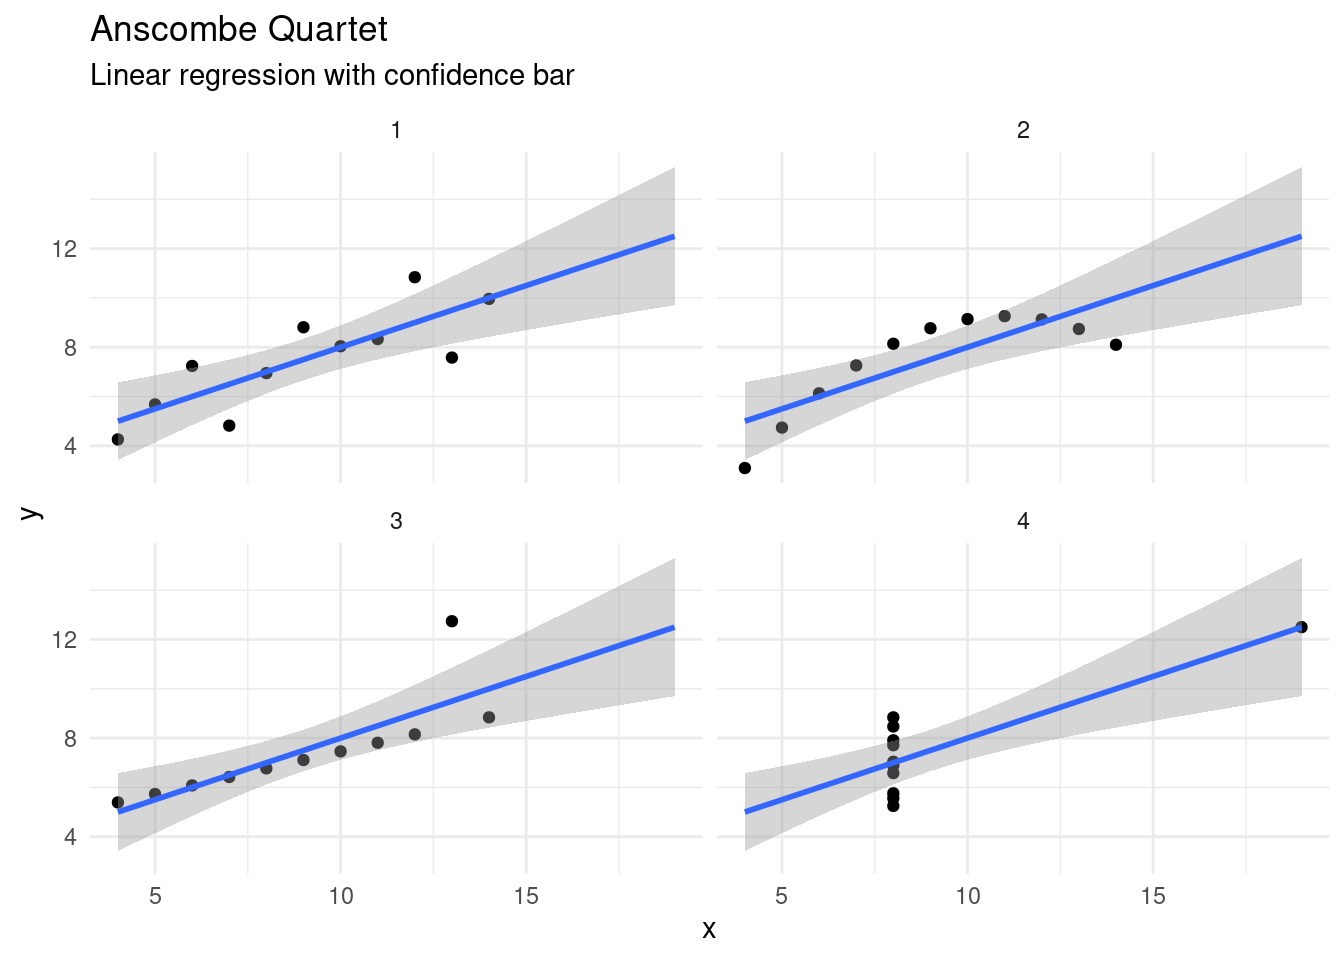
\includegraphics[width=.7\textwidth]{img/intro/Anscombe_Lm_Points-1.png}
  \end{center}

  \footnotesize
  Source : Wikipedia
\end{frame}



\section*{Use cases}

\begin{frame}{Use cases}
  \begin{columns}[c]
    
    \begin{column}{.5\textwidth}
      \begin{figure}
        \centering
        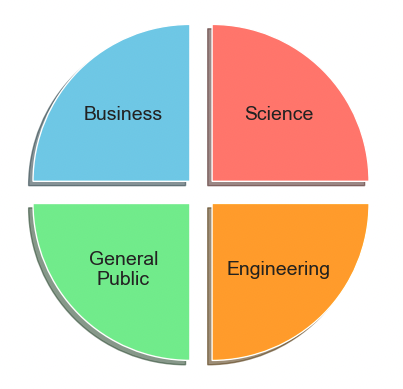
\includegraphics[width=\textwidth]{img/viz/pie-level-tech.png}
      \end{figure}
    \end{column}
    
    \begin{column}{.5\textwidth}
      \begin{itemize}
        \item Wide range of use cases
        \item Various fields
        \item Differents levels of understanding of the data visualization concepts
      \end{itemize}
    \end{column}

  \end{columns}
\end{frame}


\begin{frame}{Use cases / General public}
  \textbf{Public health}

  \centering
  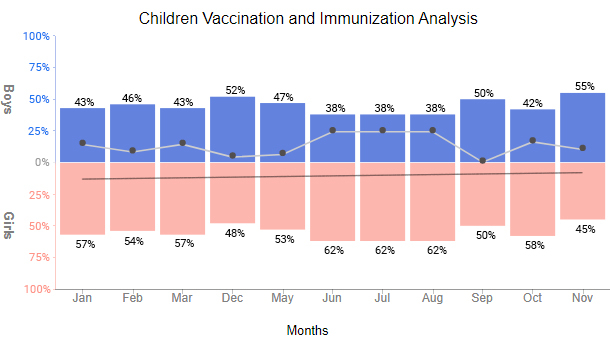
\includegraphics[width=\textwidth]{img/viz/uc-healthcare.jpg}

% ref: https://chartexpo.com/blog/healthcare-data-visualization#
\end{frame}


\begin{frame}{Use cases / General public}
  \textbf{Statistics about populations}

  \centering
  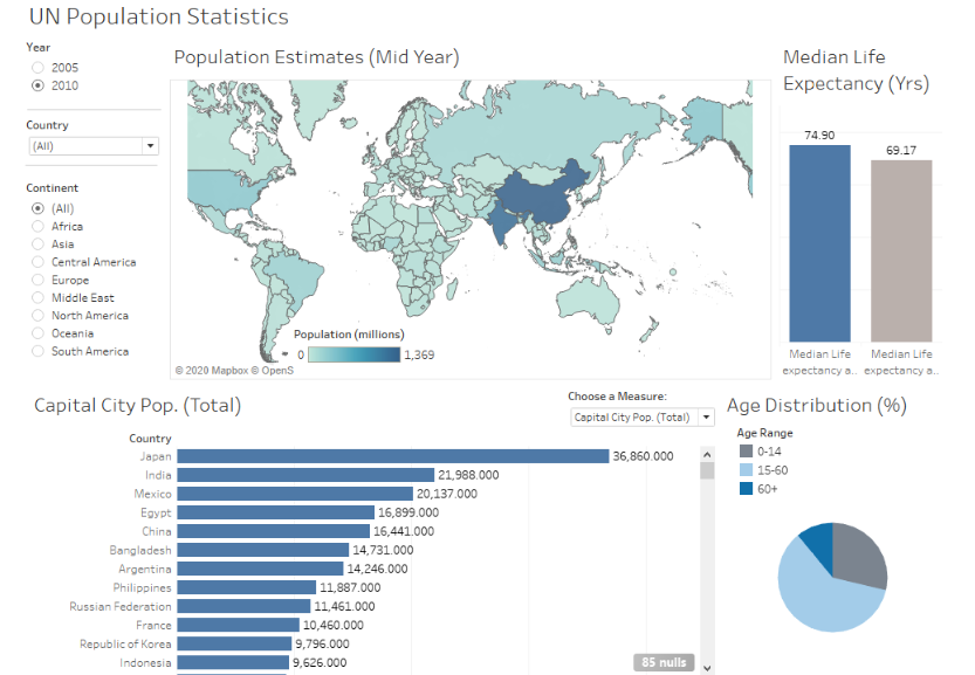
\includegraphics[width=\textwidth]{img/viz/uc-population.png}

  % Ref: https://www.linkedin.com/pulse/visualizing-un-population-data-ruth-cheng/
\end{frame}

\begin{frame}{Use cases / General public}
  \textbf{Environmental and climate change}

  \centering
  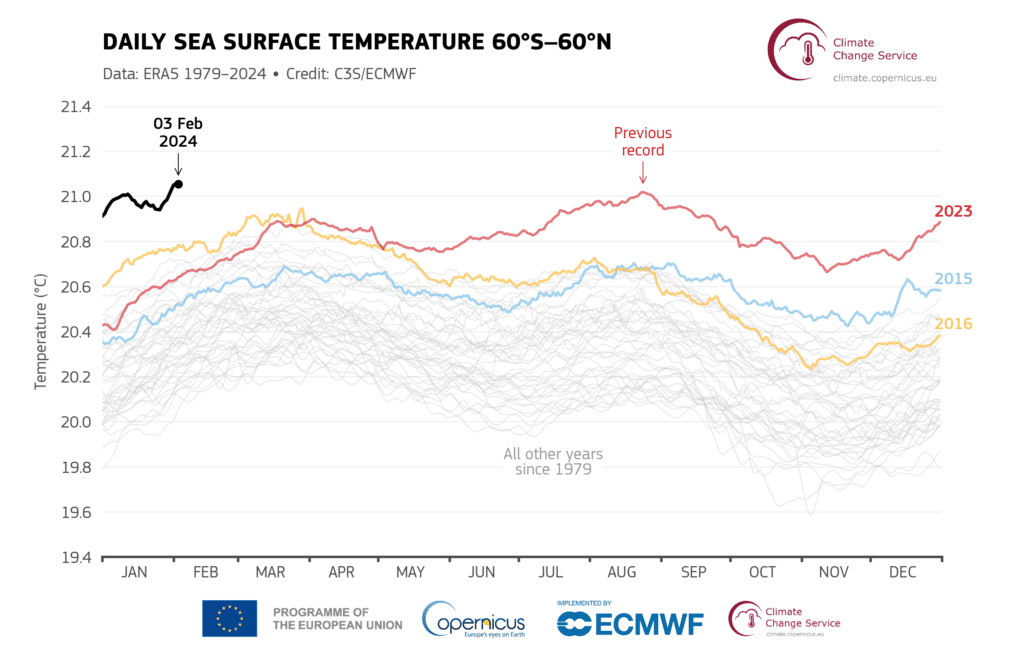
\includegraphics[width=\textwidth]{img/viz/uc-climate.png}
\end{frame}



\begin{frame}{Use cases / Business}
  \textbf{Business Intelligence (BI) and Analytics}

  \centering
  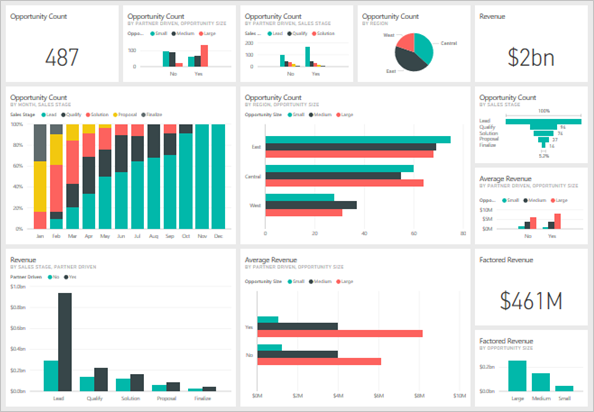
\includegraphics[width=\textwidth]{img/viz/Power_BI_dashboard.png}
\end{frame}

\begin{frame}{Use cases / Business}
  \textbf{Finance}

  \centering
  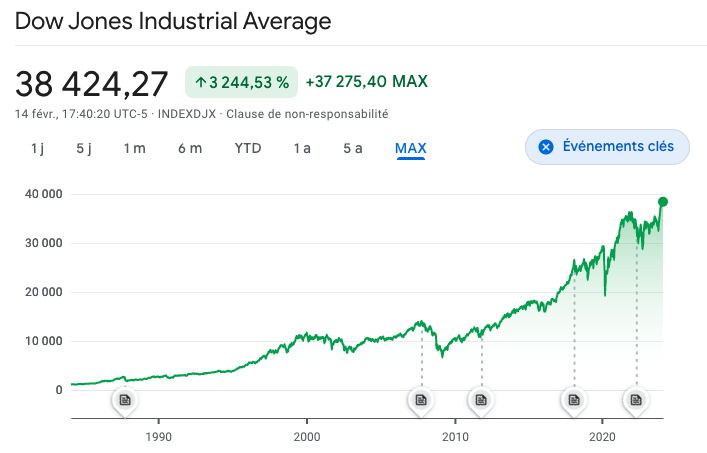
\includegraphics[width=\textwidth]{img/viz/uc-finance.png}
\end{frame}

\begin{frame}{Use cases / Business}
  \textbf{Project management}

  \centering
  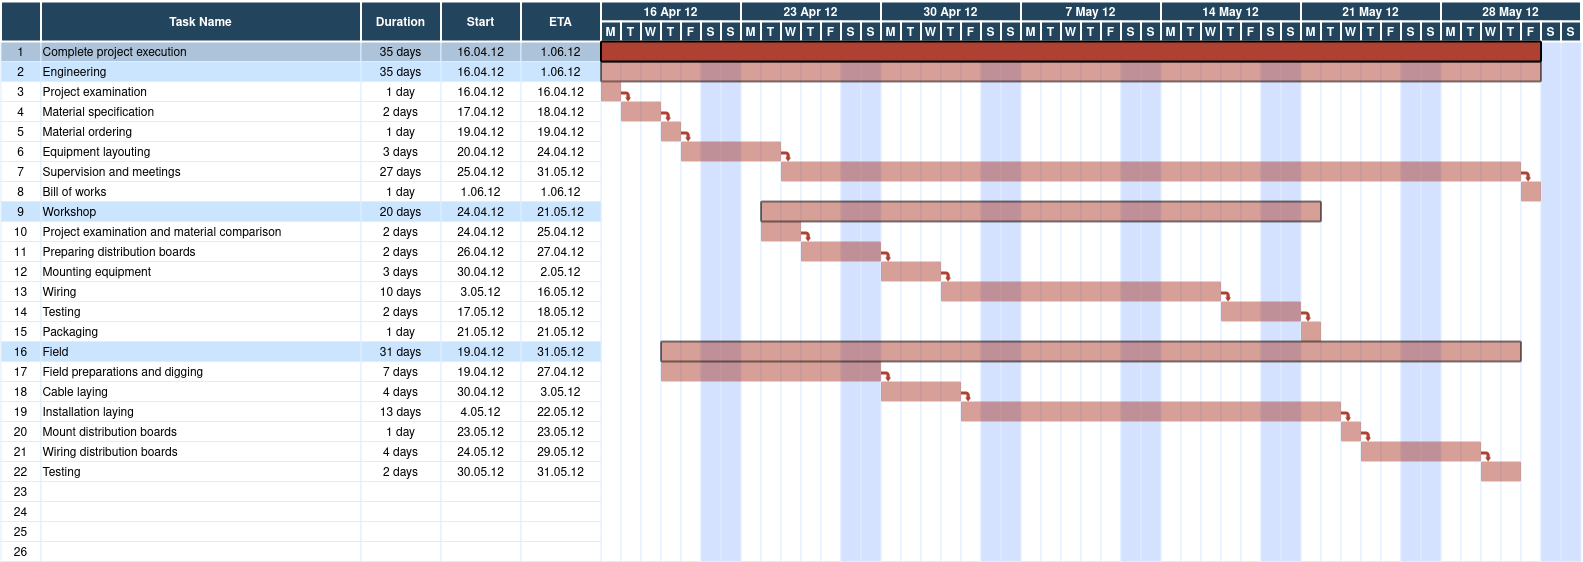
\includegraphics[width=\textwidth]{img/viz/gantt.png}
\end{frame}

\begin{frame}{Use cases / Business}
  \textbf{Team management}

  \centering
  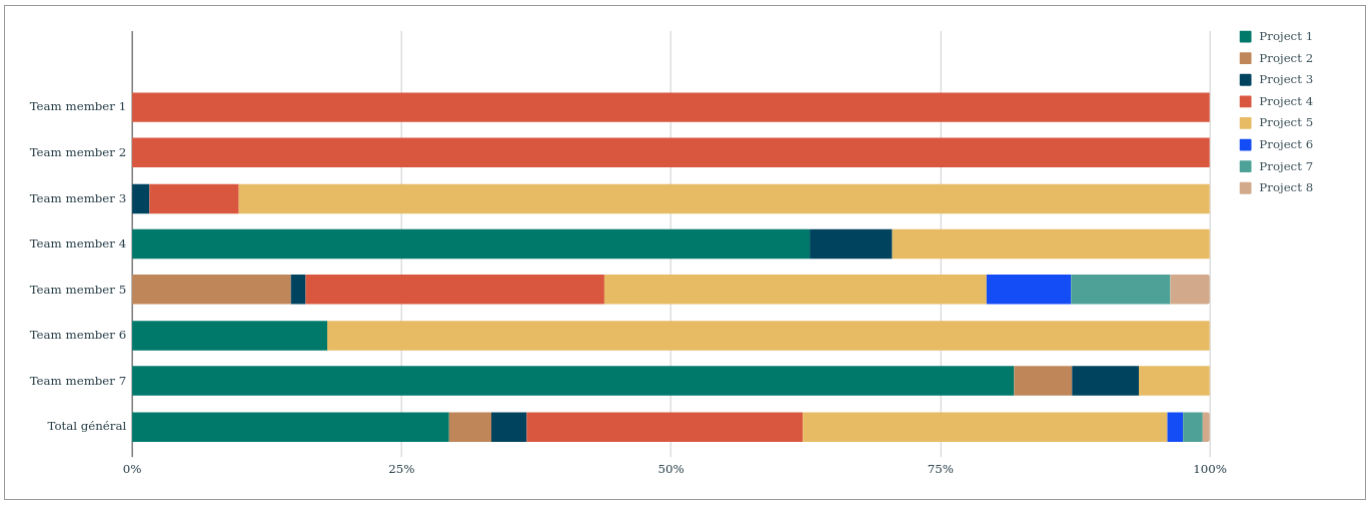
\includegraphics[width=\textwidth]{img/viz/time_tracking.png}
\end{frame}


\begin{frame}{Use cases / Engineering}
  \textbf{Anomaly detection}

  \centering
  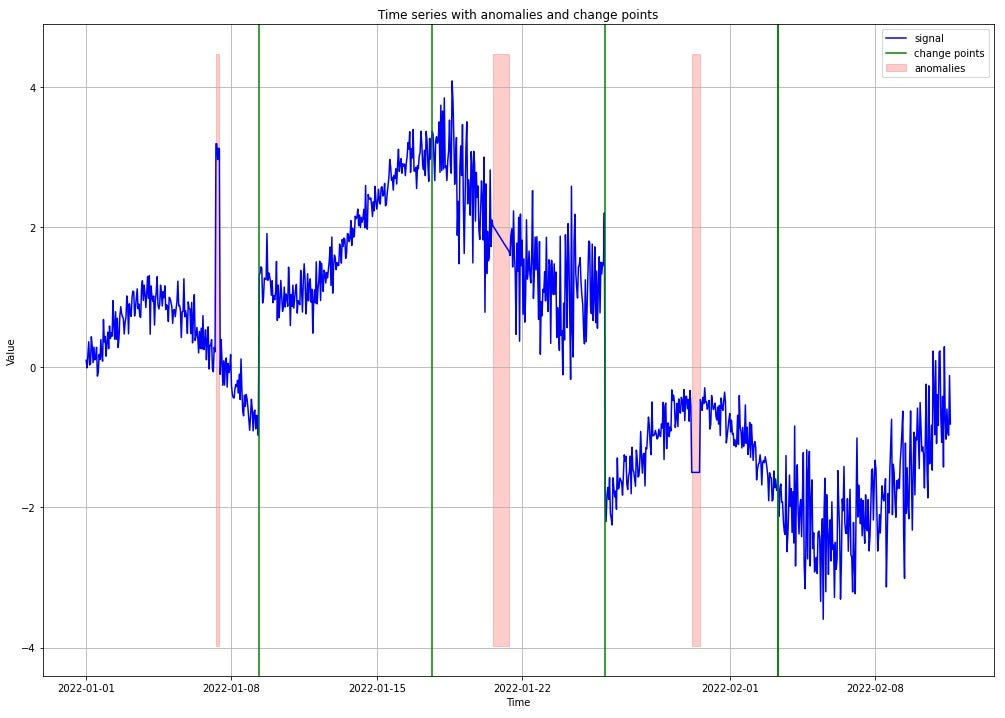
\includegraphics[width=\textwidth]{img/viz/uc-anomaly.jpg}

\end{frame}


\begin{frame}{Use cases / Engineering}
  \textbf{Urban Planning and Transportation}

  \centering
  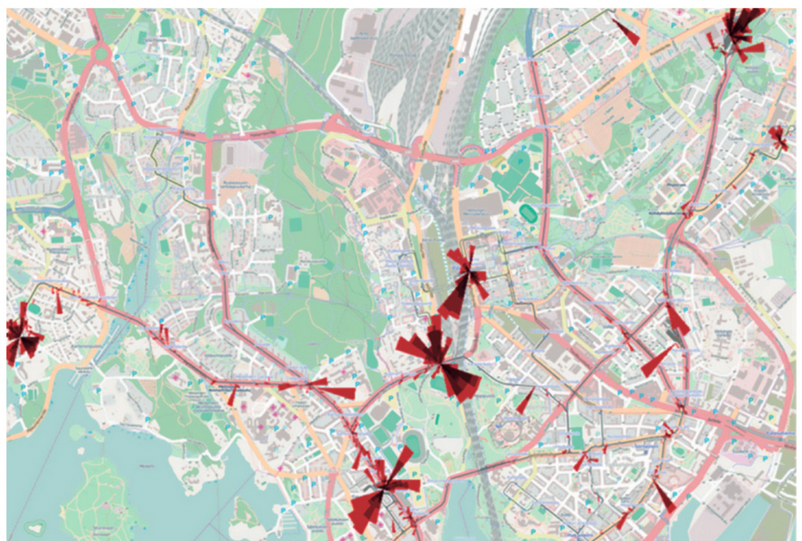
\includegraphics[width=\textwidth]{img/viz/uc-transport.png}
  % ref: https://www.mdpi.com/1424-8220/19/2/332
\end{frame}
 
\begin{frame}{Use cases / Science}
  \textbf{Data science and Machine learning}

  \centering
  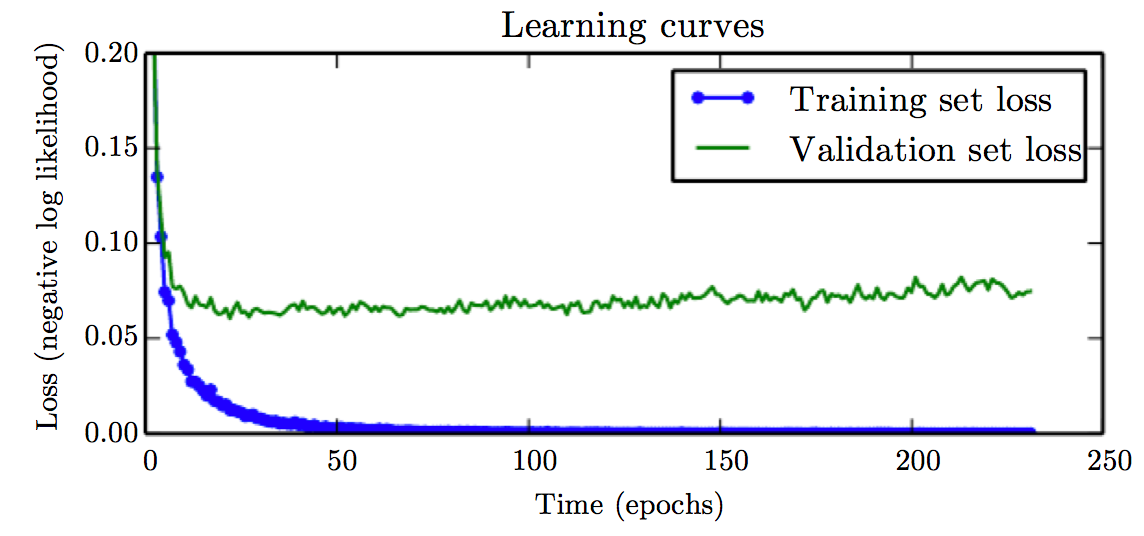
\includegraphics[width=\textwidth]{img/viz/early-stopping.png}
\end{frame}

\begin{frame}{Use cases / Science}
  \textbf{Data analysis}

  \centering
  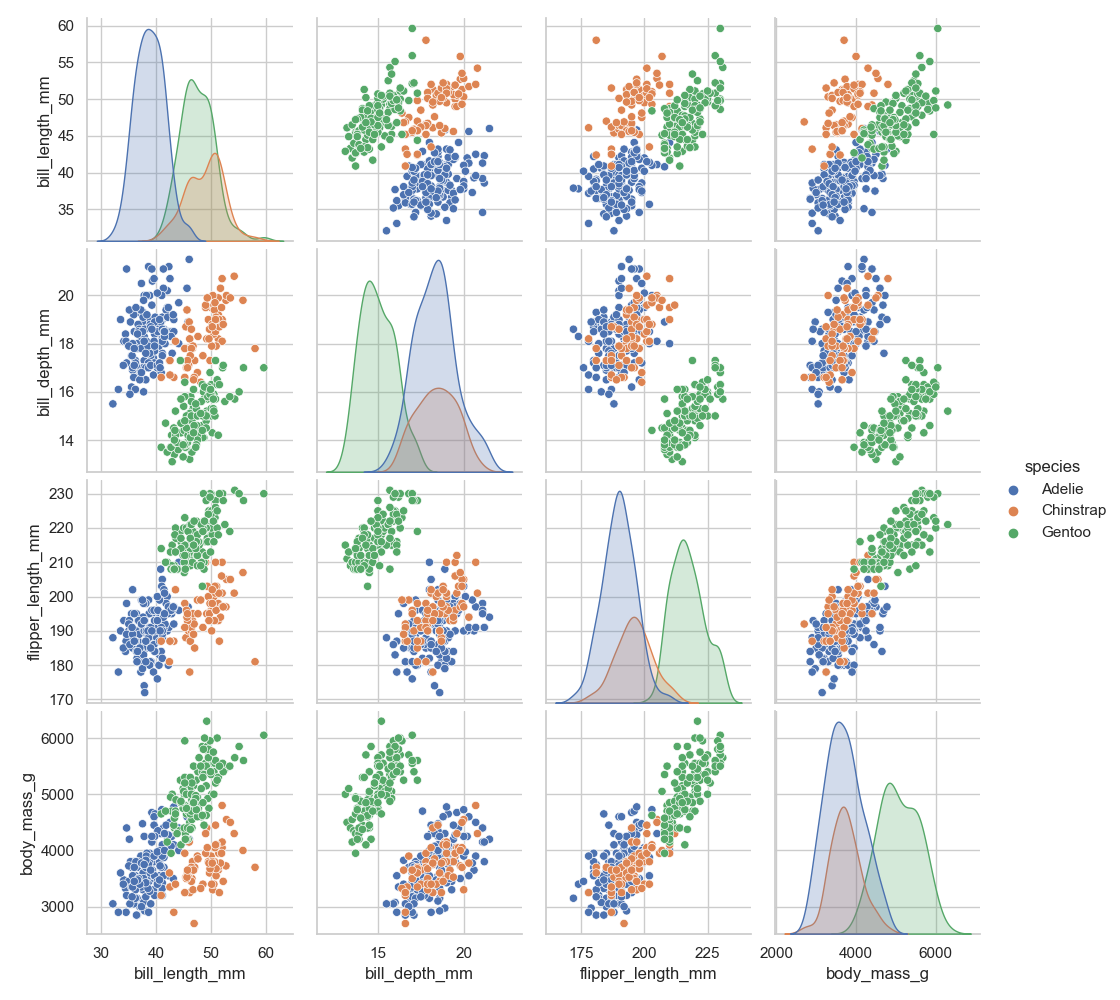
\includegraphics[width=0.8\textwidth]{img/viz/scatterplot_matrix_2.png}
\end{frame}

\begin{frame}{Use cases / Science}
  \textbf{Big data analysis}

  \centering
  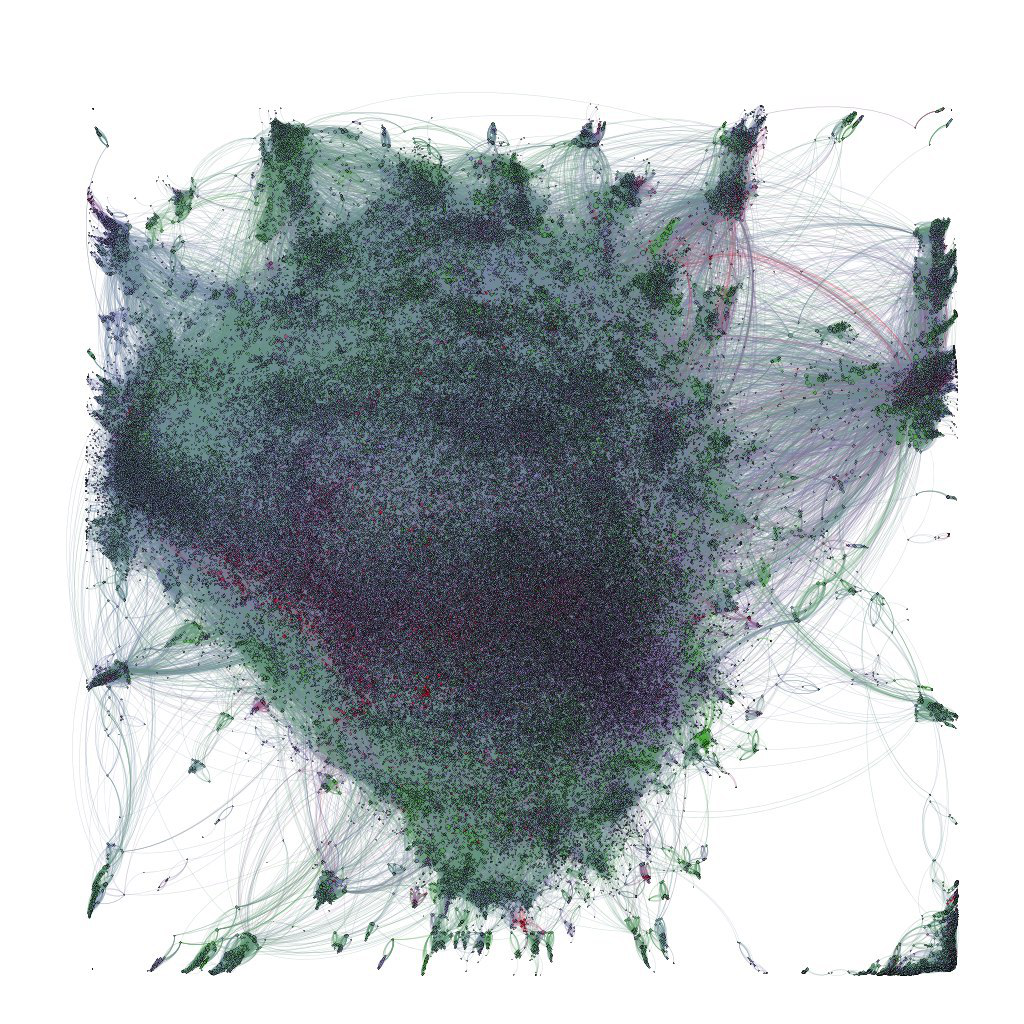
\includegraphics[width=0.8\textwidth]{img/viz/large_graph.png}
\end{frame}


\section*{Softwares}

\begin{frame}{Softwares}
  \centering
  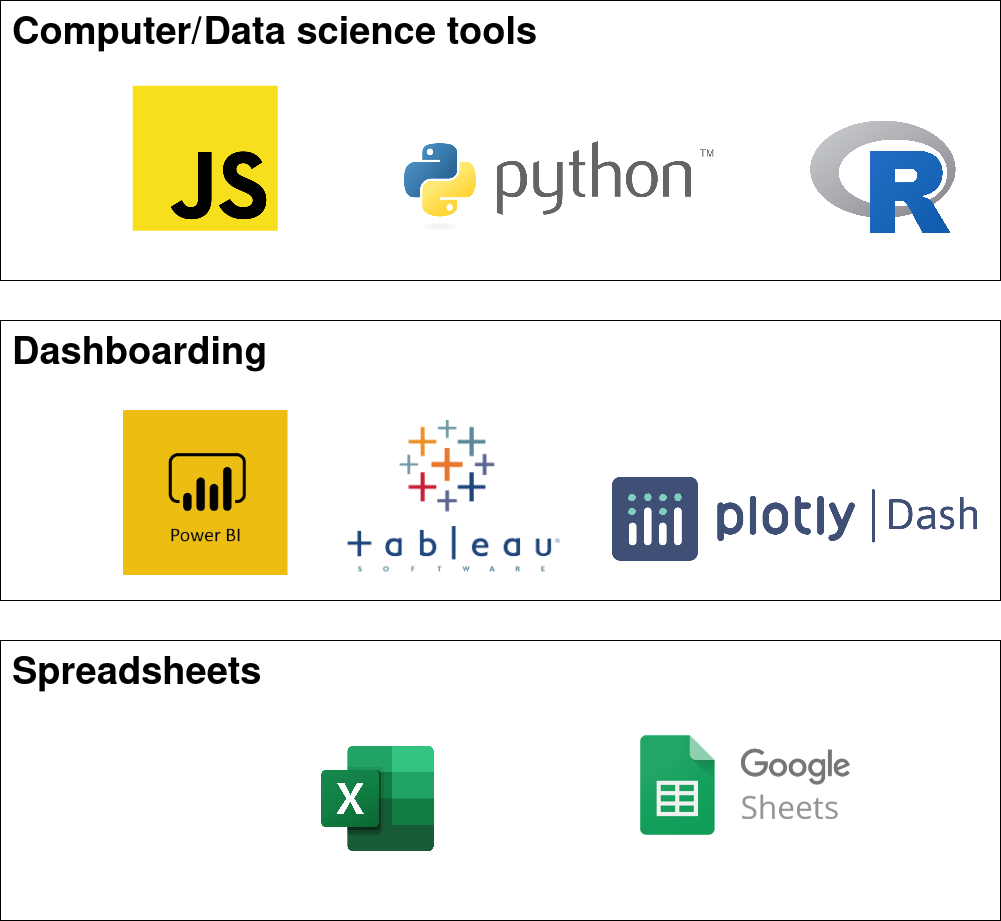
\includegraphics[width=0.7\textwidth]{img/viz/softwares.png}
\end{frame}



\section*{Best practices for Effective Data Visualization}

\begin{frame}{Best practice 1}

  \begin{block}{Consider your audience}
    \medskip
    \begin{itemize}
      \item Adapt your visualization to people
      \item Understand your audience’s area of expertise,
      \item[\textcolor{white}{x}] level of technical knowledge, and interests
    \end{itemize}
  \end{block}

  \bigskip

  \begin{columns}
    \begin{column}{.33\textwidth}
      
\includegraphics[width=\textwidth]{img/viz/BestPractice.png}
    \end{column}

    \begin{column}{.66\textwidth}
    \end{column}
  \end{columns}


\end{frame}

\begin{frame}{Best practice 2}
  
  \begin{block}{Clear the clutter}
    \medskip
    \begin{itemize}
      \item Avoid making unreadable, cluttered visualizations
      \item Ask yourself if what you’re including is relevant to the audience
      \item Remove unnecessary elements as much as you can
    \end{itemize}
  \end{block}

  \bigskip

  \begin{columns}
    \begin{column}{.33\textwidth}
      
\includegraphics[width=\textwidth]{img/viz/BestPractice.png}
    \end{column}

    \begin{column}{.66\textwidth}
    \end{column}
  \end{columns}
\end{frame}

\begin{frame}{Best practice 3}
  
  \begin{block}{Keep an eye on the fonts}
    \medskip
    \begin{itemize}
      \item One font with no more than three different sizes
      \item Respect the font hierarchy, keep headings larger than the body
      \item Use a bold typeface to highlight \textbf{key elements} and headings
    \end{itemize}
  \end{block}

  \bigskip

  \begin{columns}
    \begin{column}{.33\textwidth}
      
\includegraphics[width=\textwidth]{img/viz/BestPractice.png}
    \end{column}

    \begin{column}{.66\textwidth}
    \end{column}
  \end{columns}
\end{frame}


  
\begin{frame}{Best practice 4}
  
  \begin{block}{Use colors creatively}
    \medskip
    \begin{itemize}
      \item Color is one of the most eye-catching aspects of data visualization
      \item Choose a color scheme of your data visualization
      \item Use colors to hightlight groups, levels of importance, etc.
    \end{itemize}
  \end{block}

  \bigskip

  \begin{columns}
    \begin{column}{.33\textwidth}
      
\includegraphics[width=\textwidth]{img/viz/BestPractice.png}
    \end{column}

    \begin{column}{.66\textwidth}
    \end{column}
  \end{columns}
\end{frame}





\section*{Types of charts}

\begin{frame}{Overview}
  \centering
  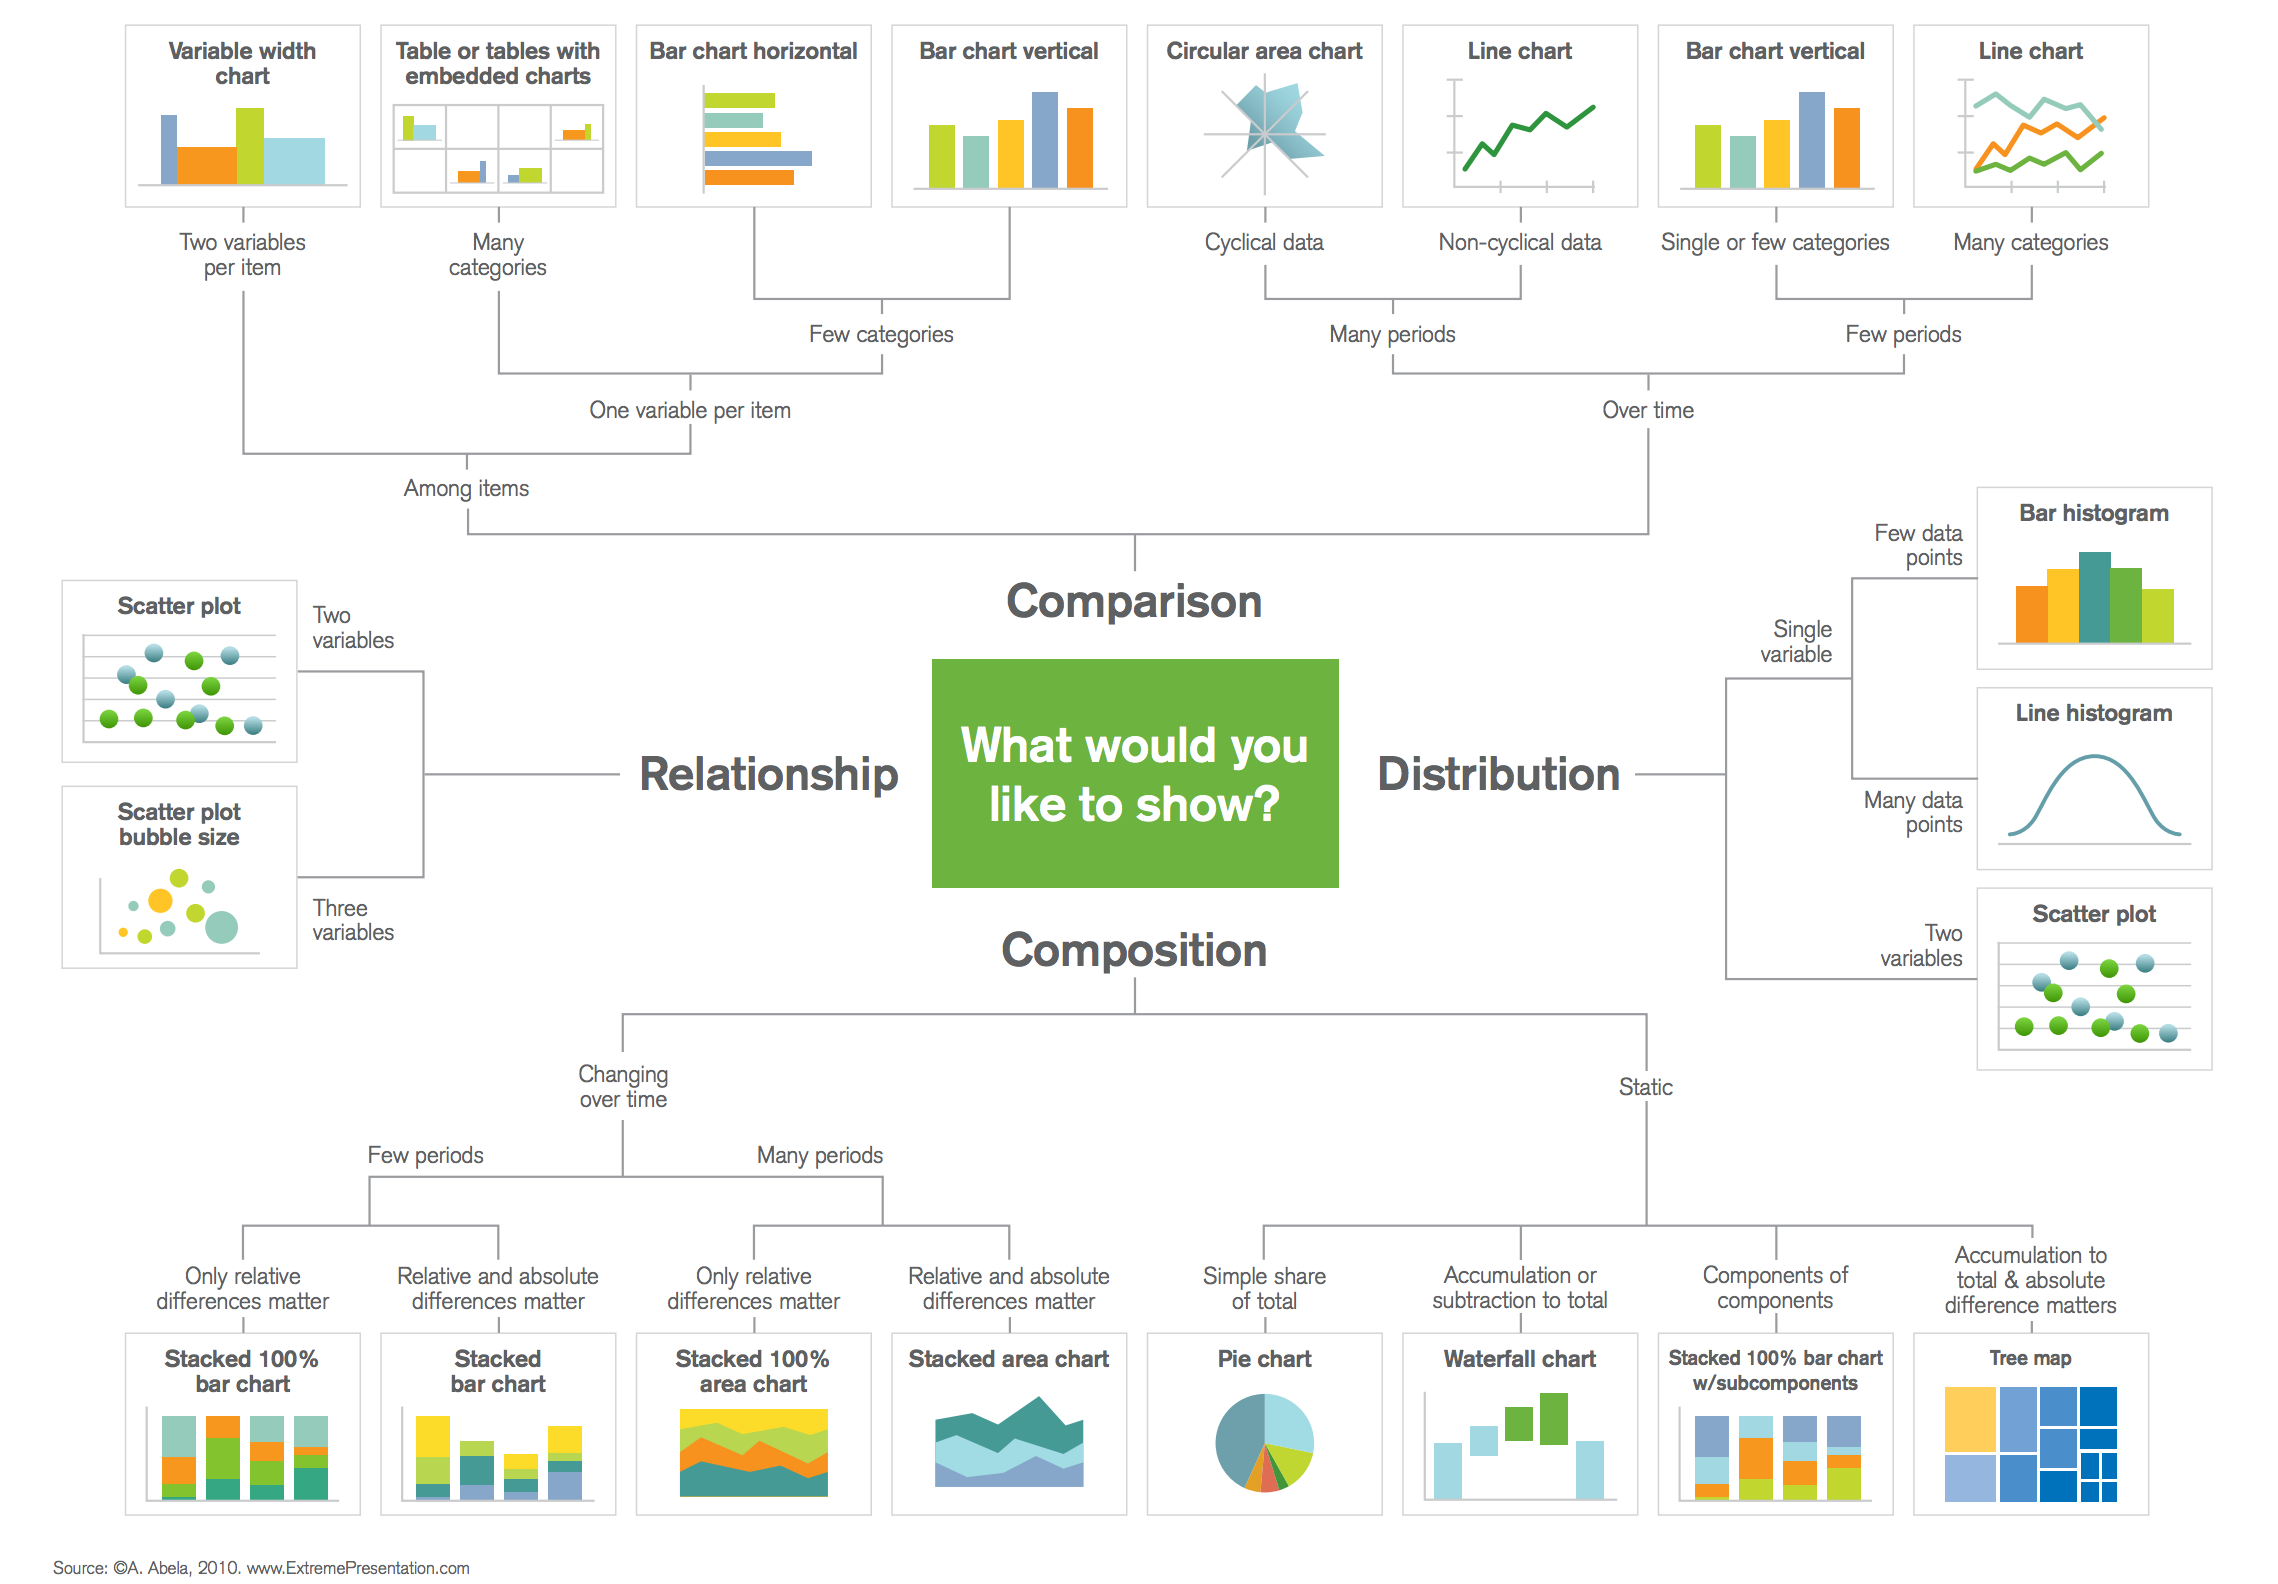
\includegraphics[width=\textwidth]{img/viz/chart-chooser-color}
\end{frame}

\begin{frame}{1D Bar chart}
  \centering
  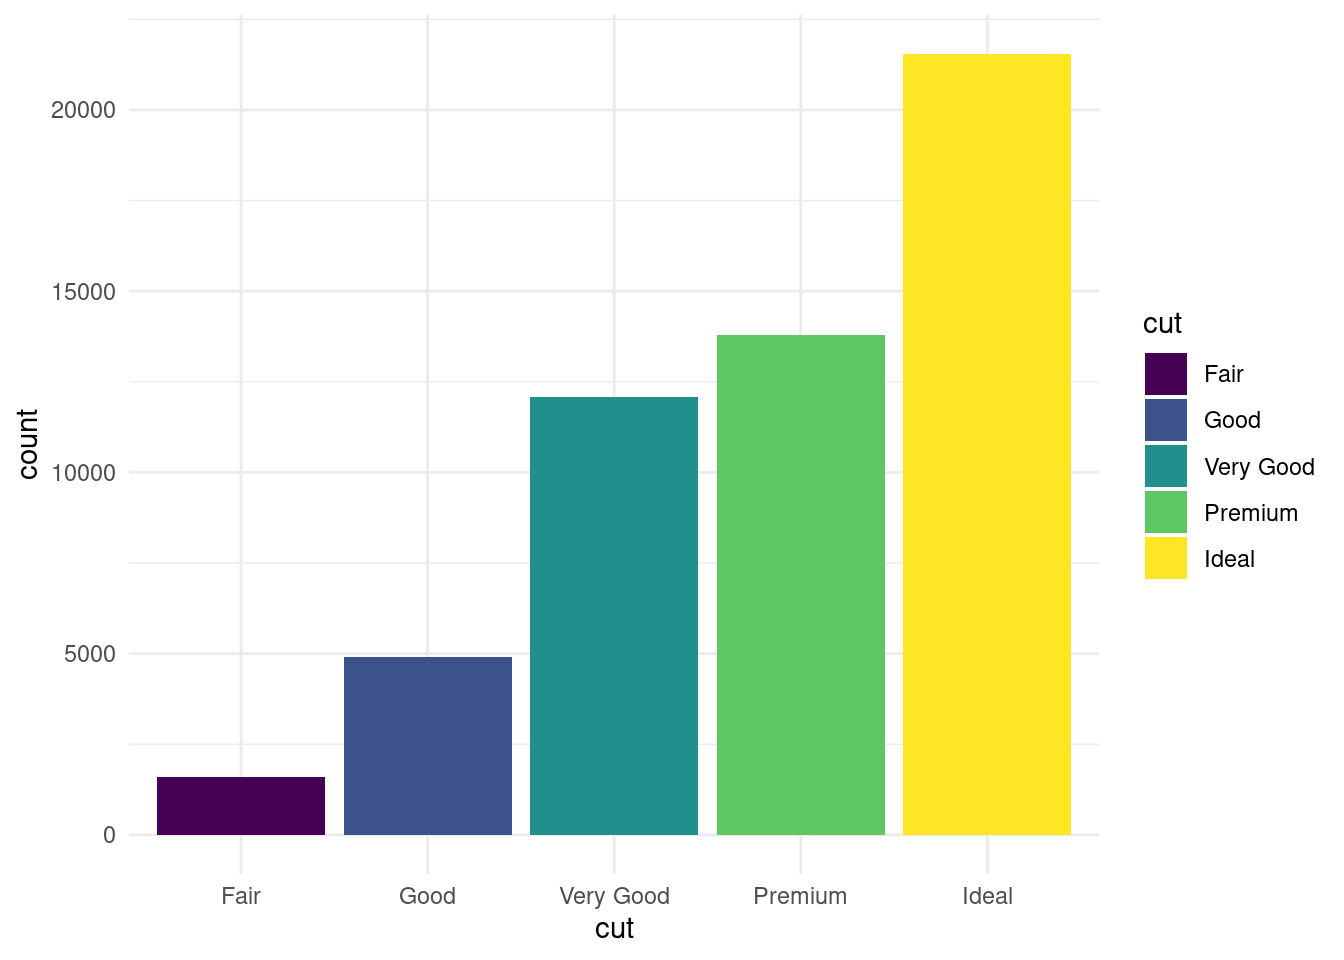
\includegraphics[width=.6\textwidth]{img/viz/barchart}
\end{frame}

\begin{frame}{1D Bar chart}
  \centering
  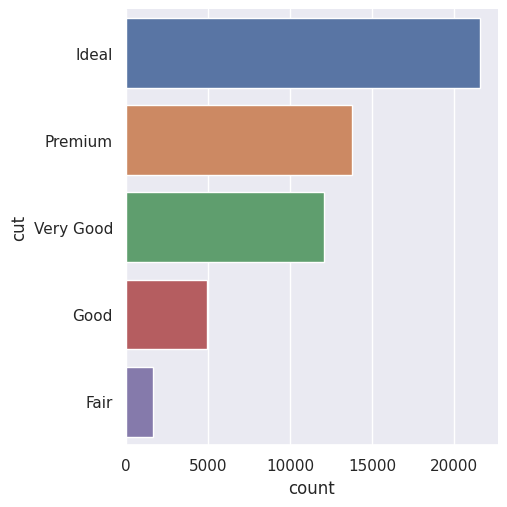
\includegraphics[width=.6\textwidth]{img/viz/catplot}
\end{frame}

\begin{frame}{1D Bar chart}
  \centering
  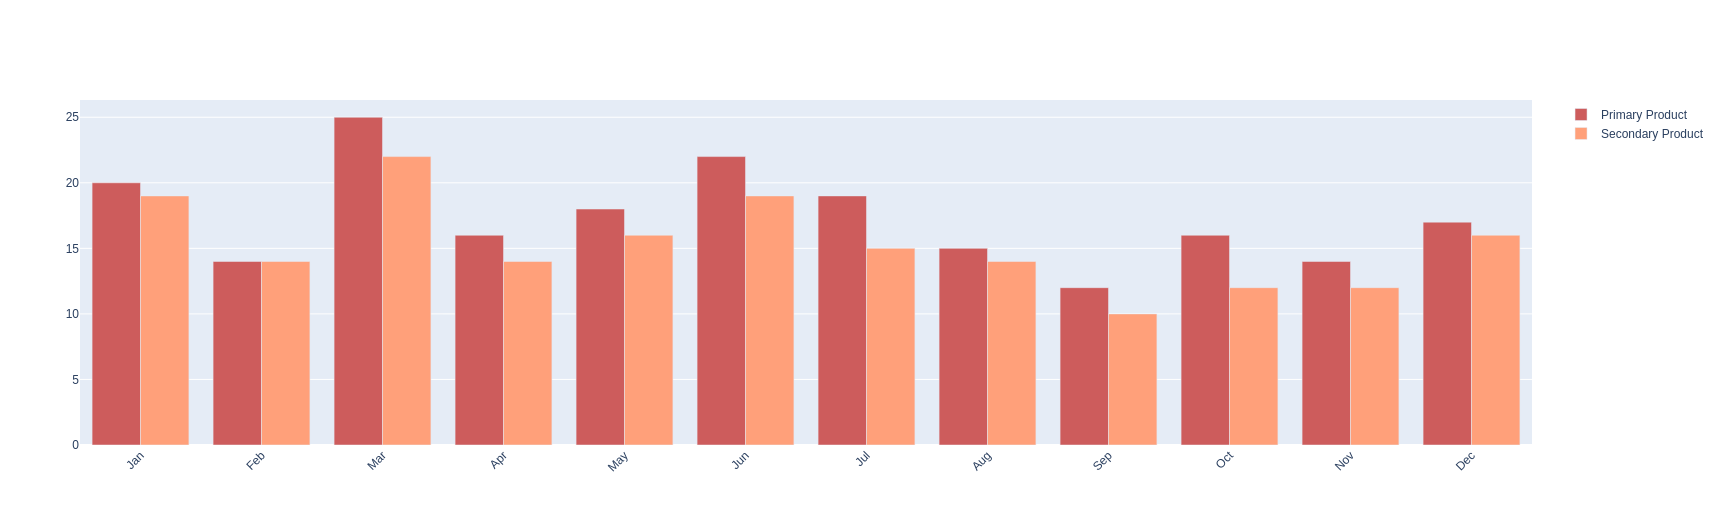
\includegraphics[width=\textwidth]{img/viz/barchart_grouped}
\end{frame}

\begin{frame}{1D Pie chart}
  \centering
  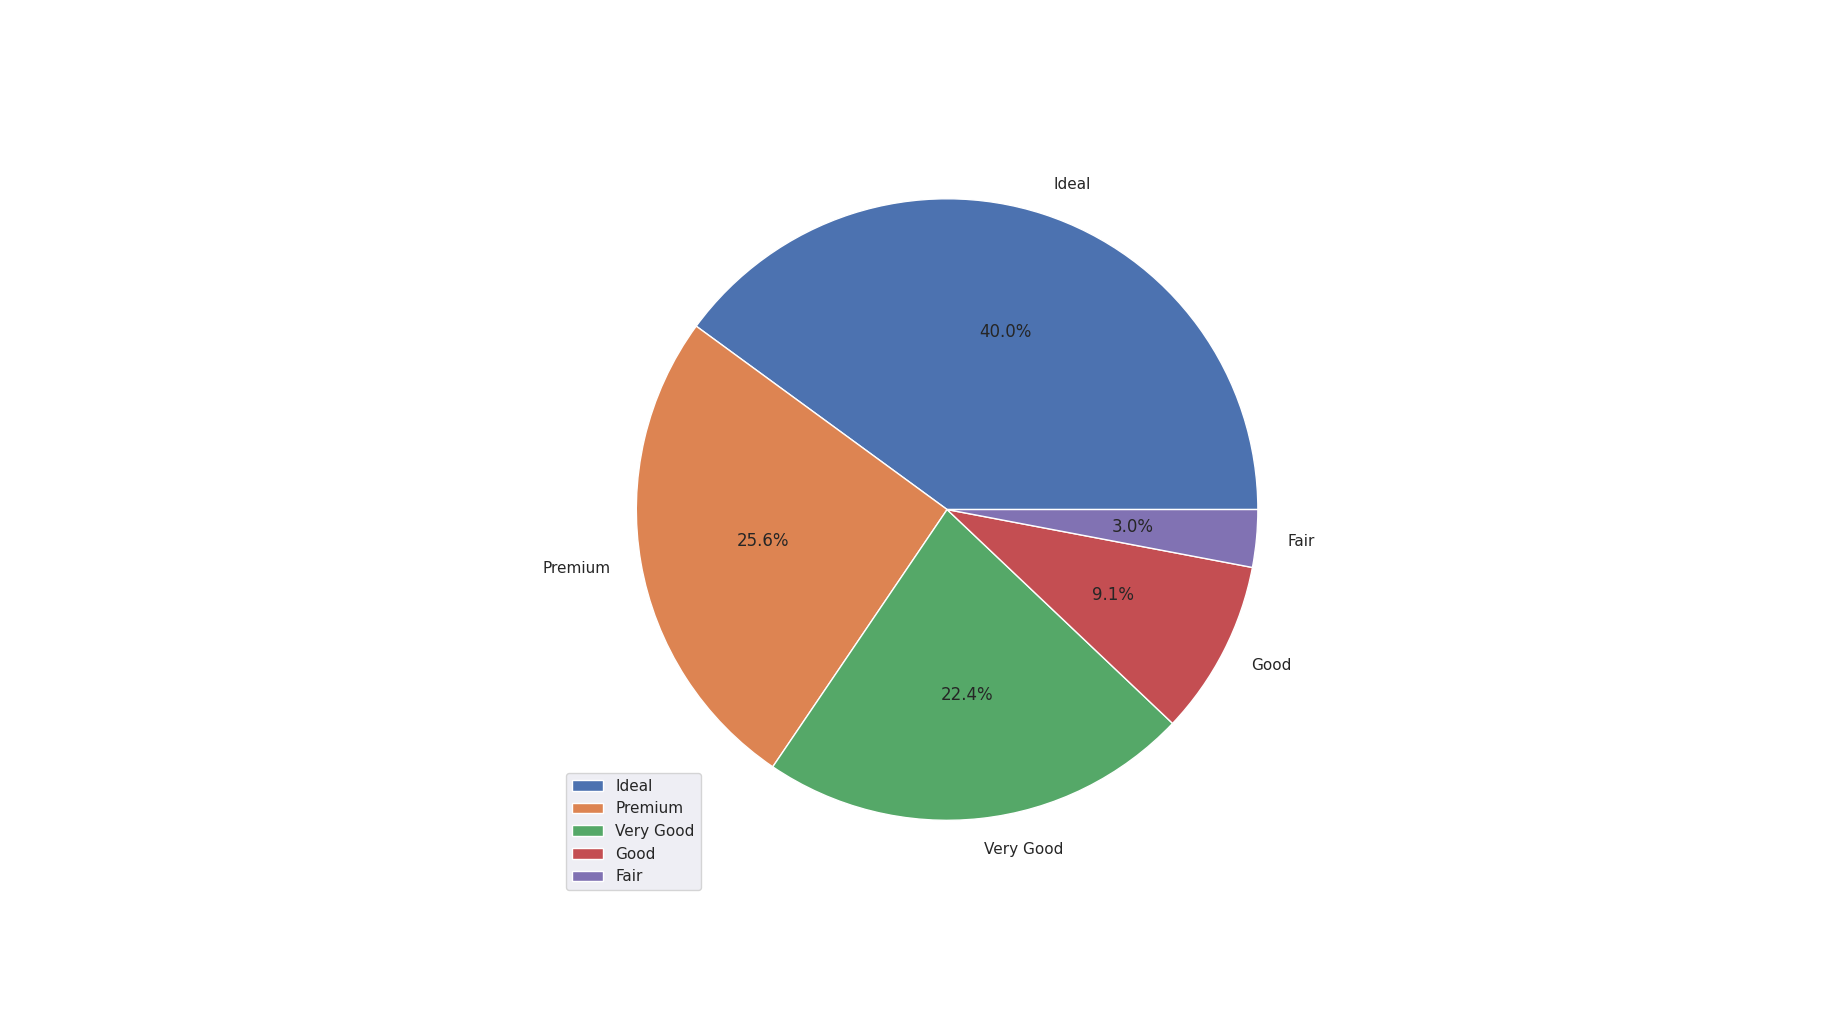
\includegraphics[width=\textwidth]{img/viz/pie}
\end{frame}

\begin{frame}{1D Pie and bar chart combined}
  \centering
  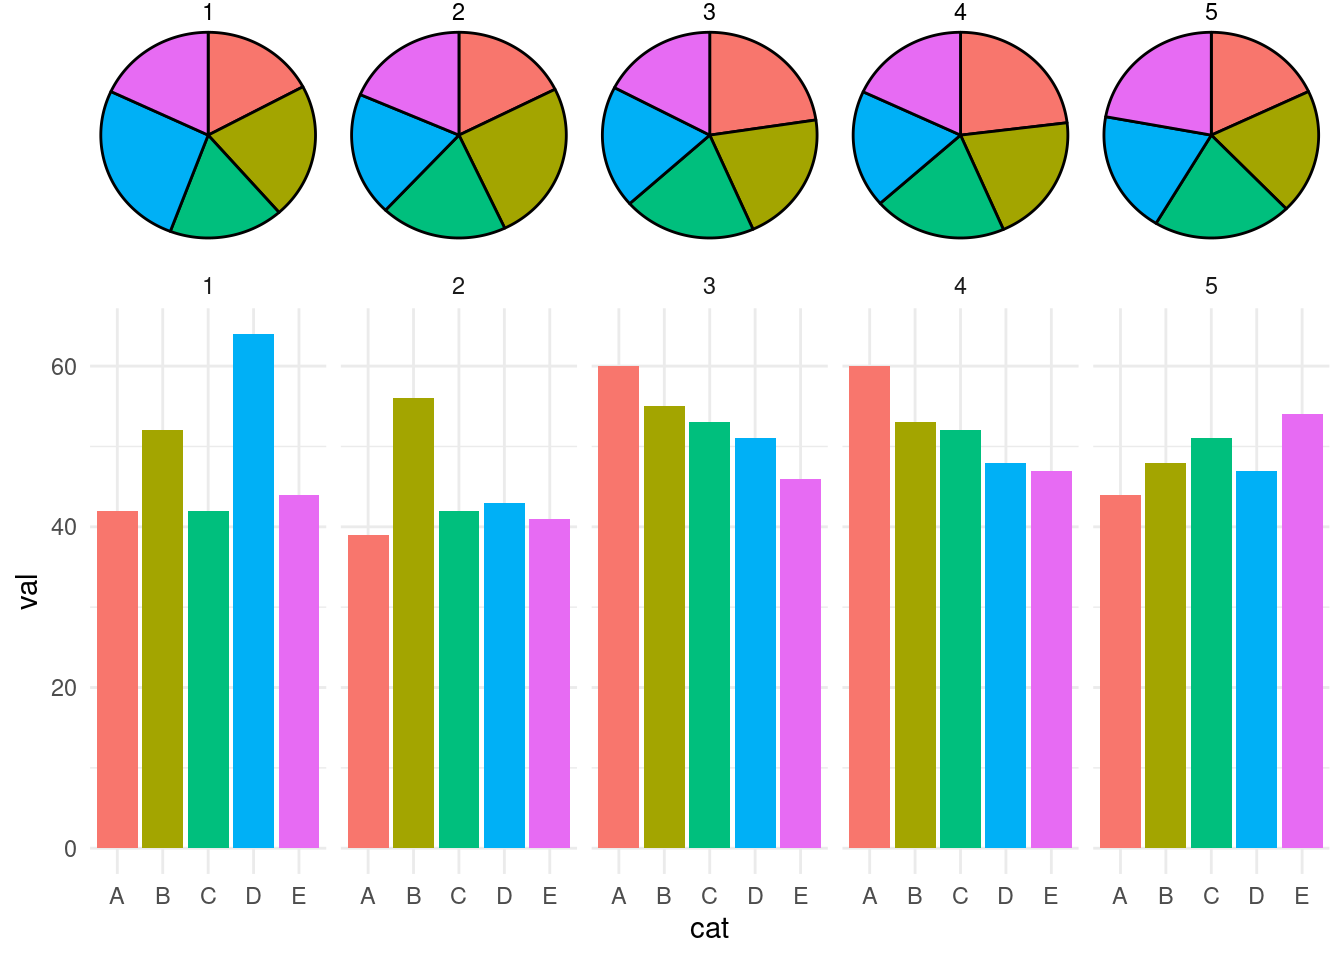
\includegraphics[width=.6\textwidth]{img/viz/bar_pie}
\end{frame}


\begin{frame}{1D Distribution: histogram}
  \centering
  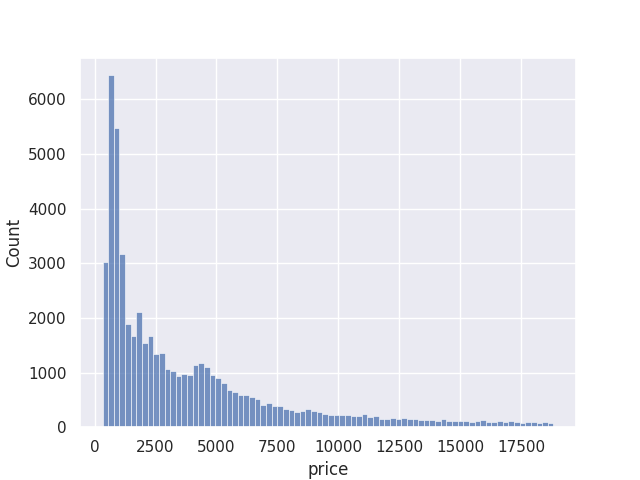
\includegraphics[width=.6\textwidth]{img/viz/histogram}
\end{frame}


\begin{frame}{1D Distribution: histogram}
  \centering
  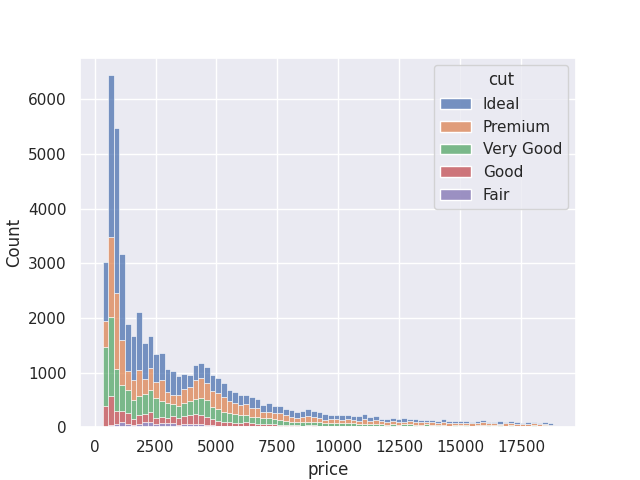
\includegraphics[width=.6\textwidth]{img/viz/hist_stacked}
\end{frame}


\begin{frame}{1D Distribution: density}
  \centering
  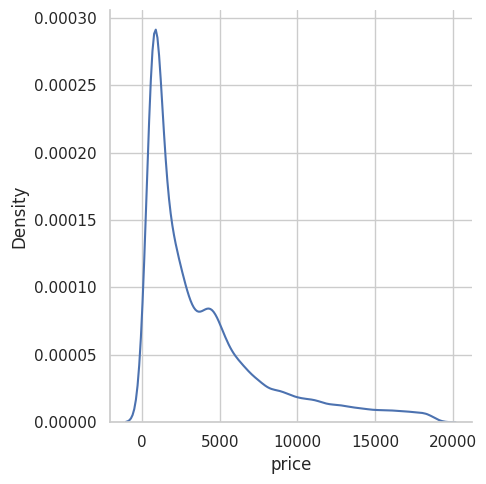
\includegraphics[width=.6\textwidth]{img/viz/kde}
\end{frame}


\begin{frame}{1D Distribution: density}
  \centering
  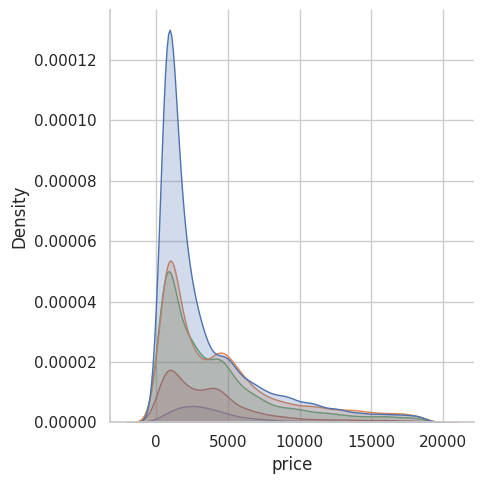
\includegraphics[width=.6\textwidth]{img/viz/kde_stacked}
\end{frame}

\begin{frame}{1D Distribution: box plot}
  \centering
  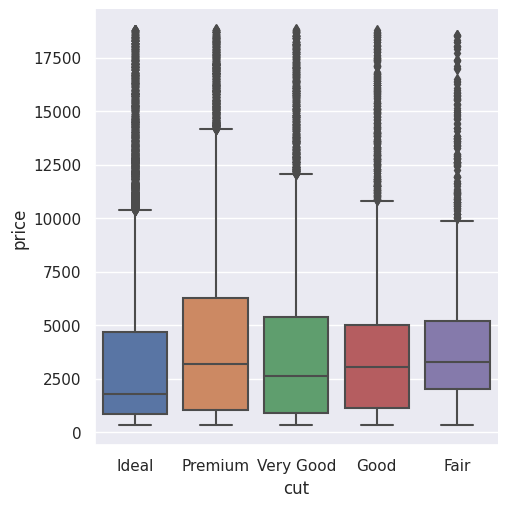
\includegraphics[width=.6\textwidth]{img/viz/box}
\end{frame}

\begin{frame}{1D Distribution: violin plot}
  \centering
  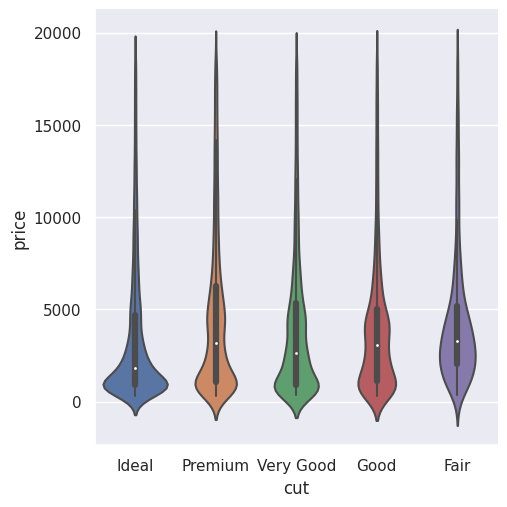
\includegraphics[width=.6\textwidth]{img/viz/violin}
\end{frame}


\begin{frame}{1D Time series}
\begin{block}{A sequence over the time}
  \centering
  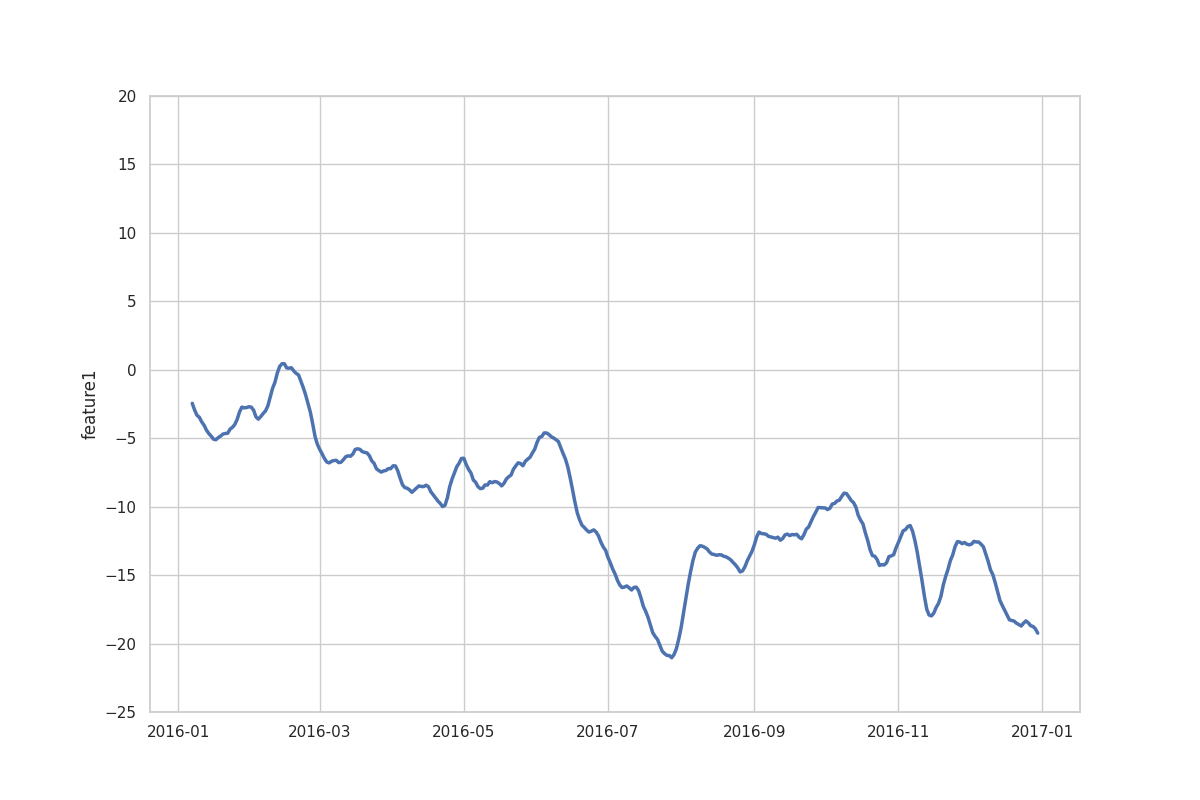
\includegraphics[width=.6\textwidth]{img/viz/line}
\end{block}
\end{frame}


\begin{frame}{1D Time series}
\begin{block}{A sequence over the time}
  \centering
  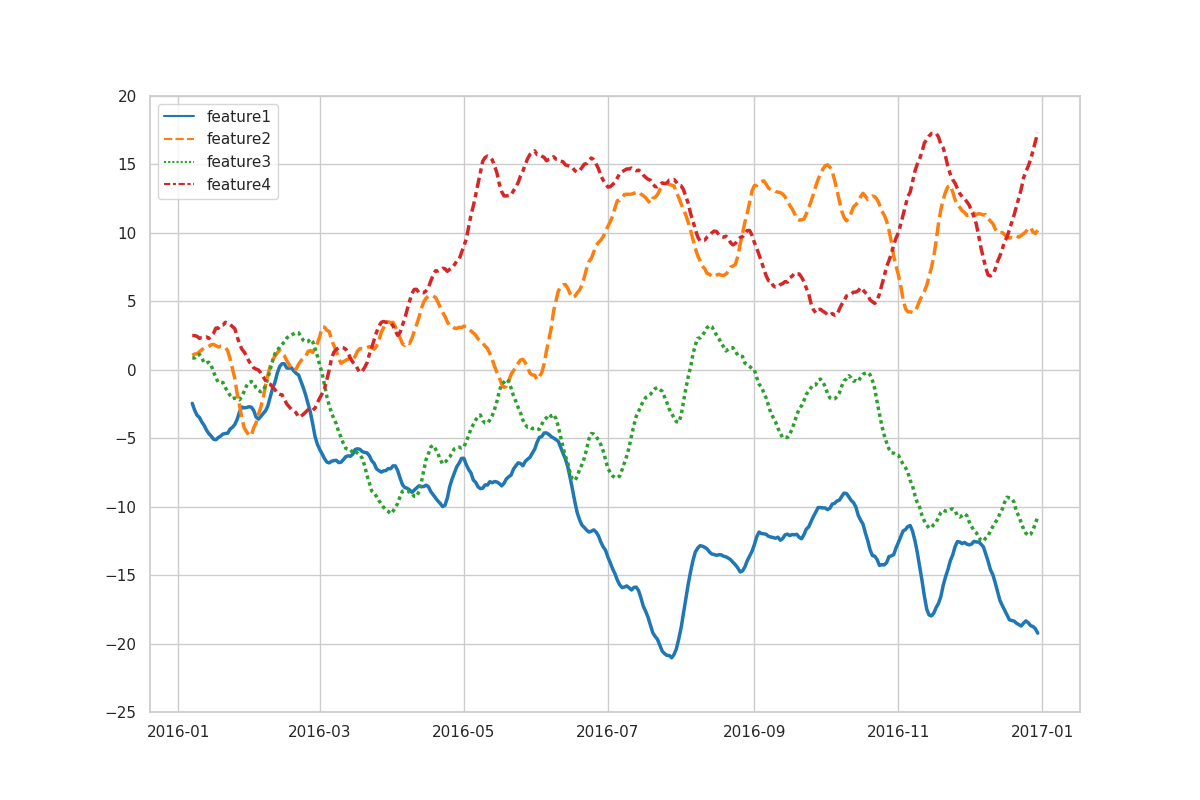
\includegraphics[width=.6\textwidth]{img/viz/line_cat}
\end{block}
\end{frame}


% 2D scatter, heatmap, pairplots, jointplot, kde

\begin{frame}{2D charts: scatter plot}
  \centering
  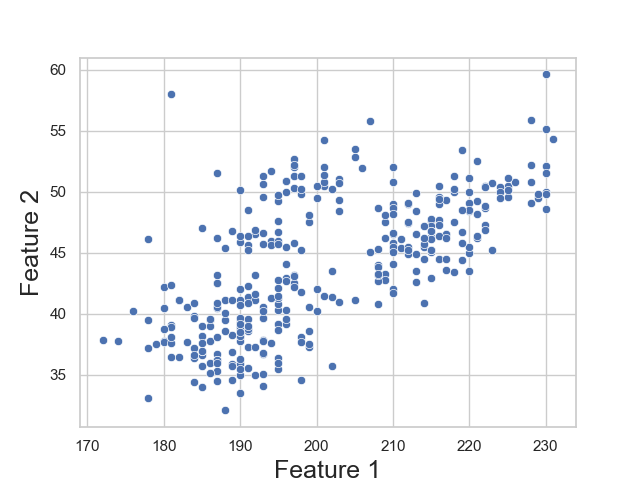
\includegraphics[width=.6\textwidth]{img/viz/scatter_2d_1}
\end{frame}

\begin{frame}{2D charts: scatter plot}
  \centering
  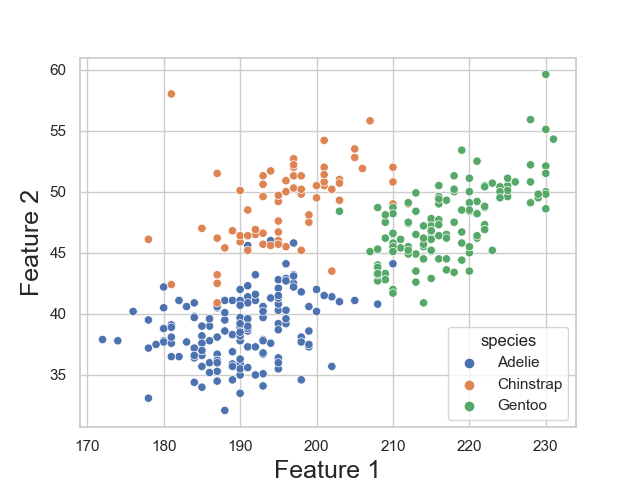
\includegraphics[width=.6\textwidth]{img/viz/scatter_2d_2}
\end{frame}

\begin{frame}{2D charts: scatter plot matrix}
  \centering
  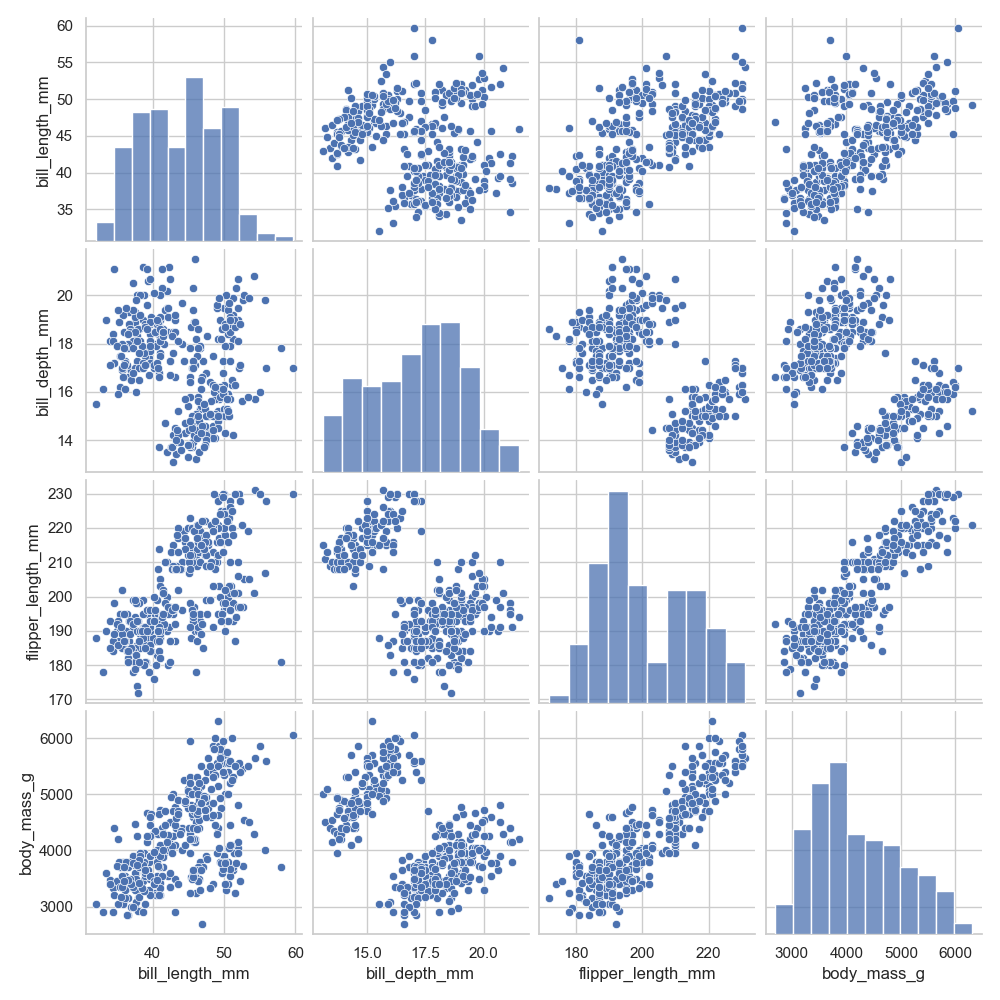
\includegraphics[width=.6\textwidth]{img/viz/scatterplot_matrix_1}
\end{frame}

  \begin{frame}{2D charts: scatter plot matrix}
    \centering
    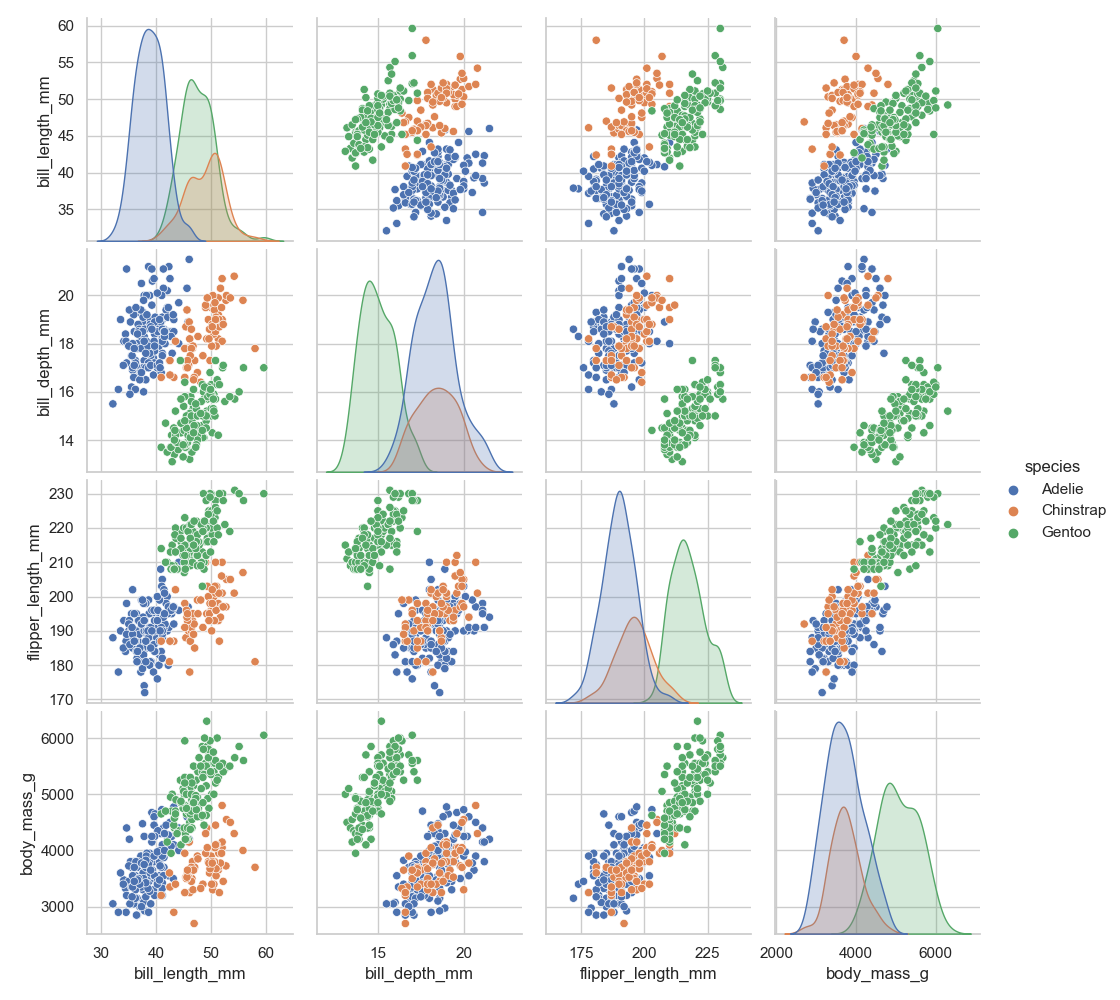
\includegraphics[width=.6\textwidth]{img/viz/scatterplot_matrix_2}
\end{frame}
      
\begin{frame}{2D charts: joint plot}
  \centering
  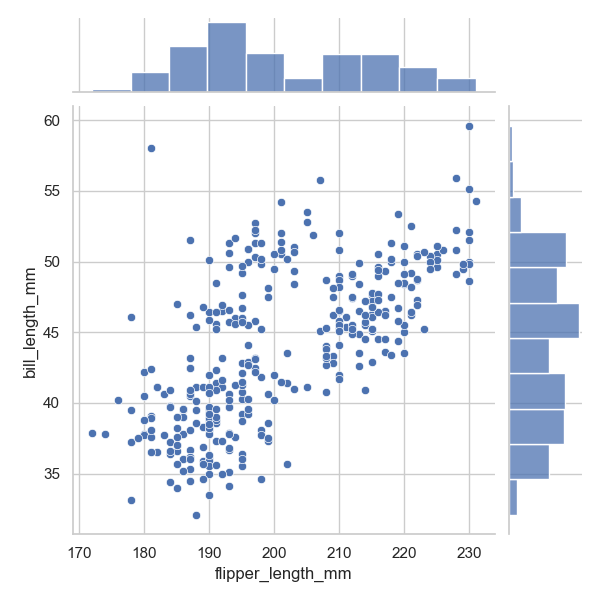
\includegraphics[width=.6\textwidth]{img/viz/jointplot_1}
\end{frame}

\begin{frame}{2D charts: joint plot}
  \centering
  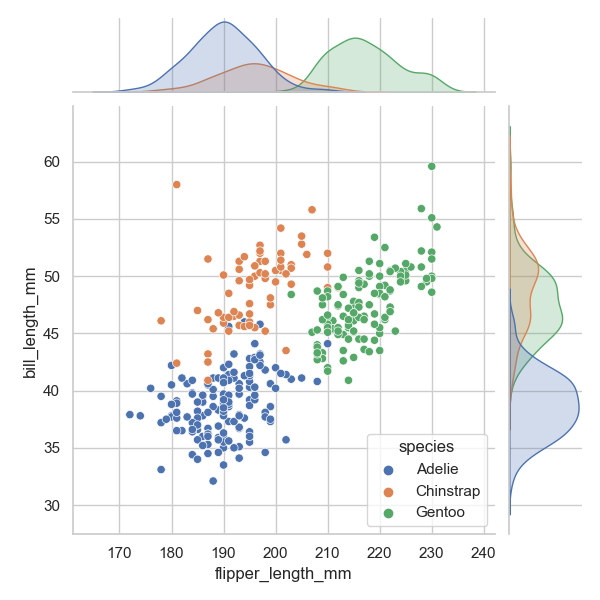
\includegraphics[width=.6\textwidth]{img/viz/jointplot_2}
\end{frame}




\begin{frame}{2D charts: heatmap}
\centering
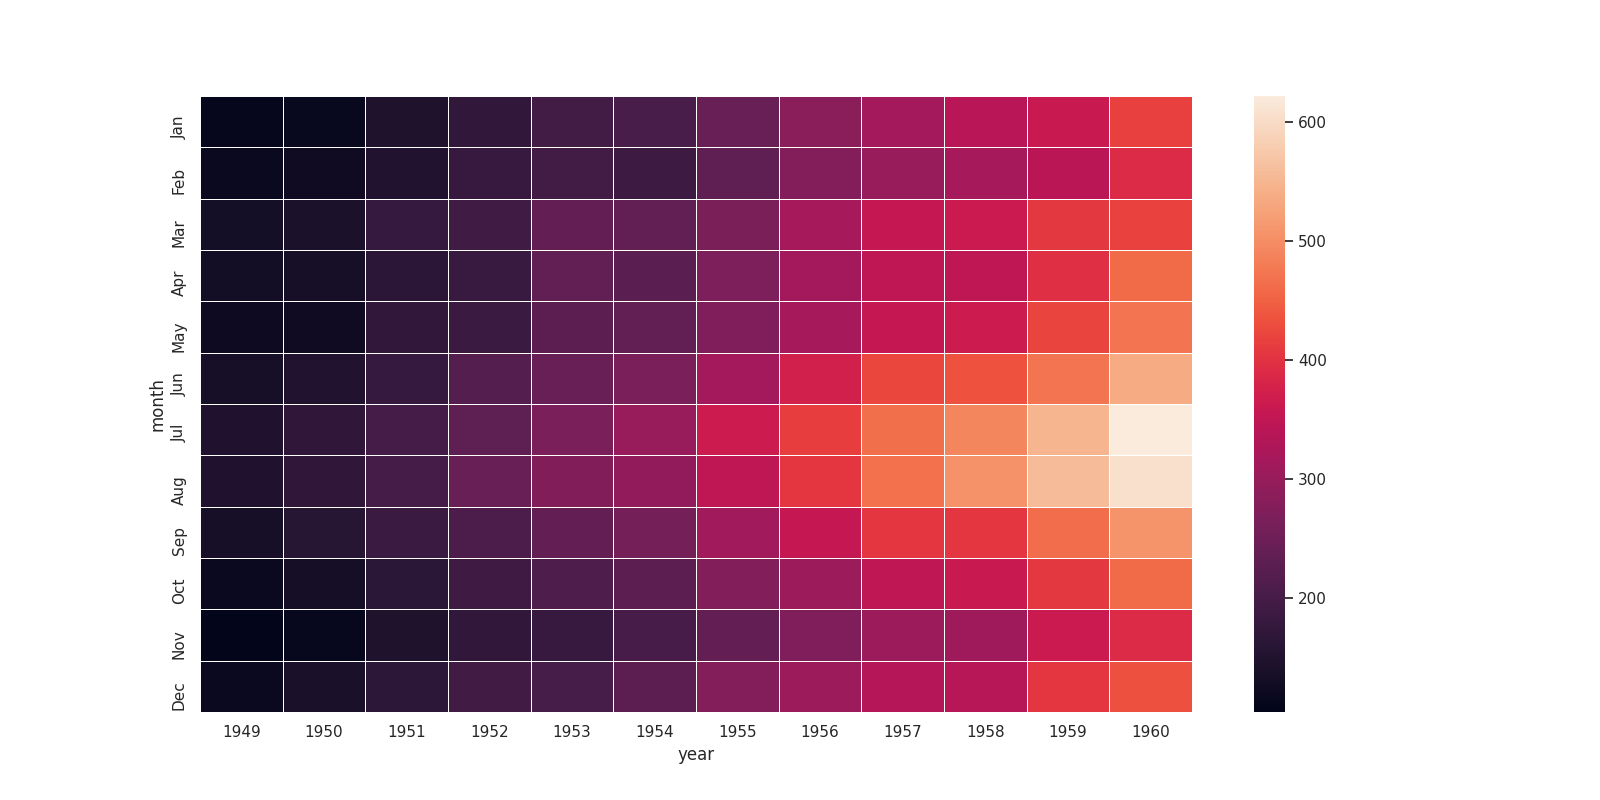
\includegraphics[width=1.2\textwidth]{img/viz/heatmap}
\end{frame}

\begin{frame}{2D charts: heatmap}
\centering
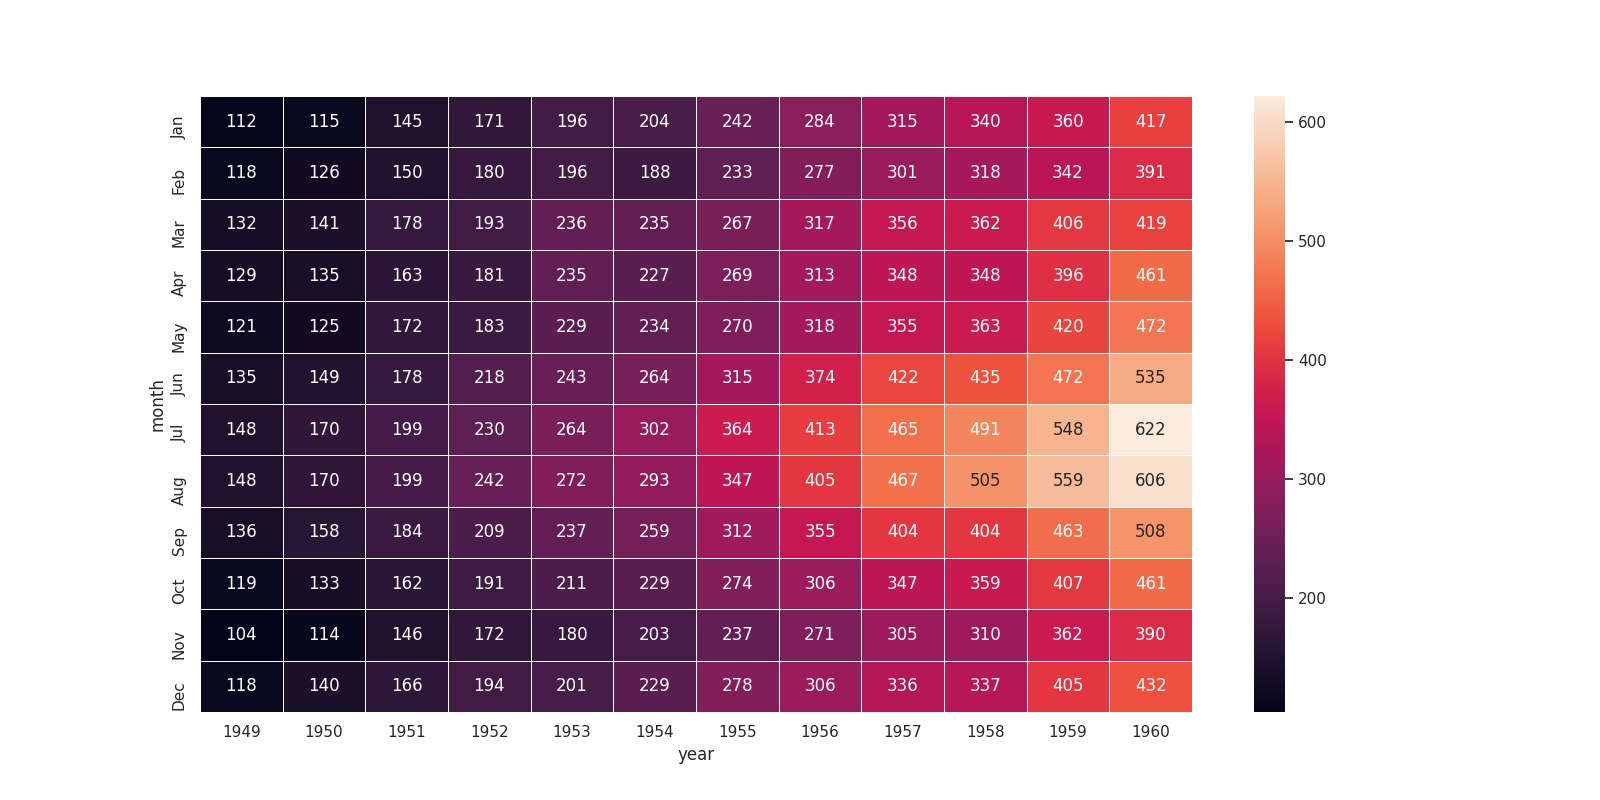
\includegraphics[width=1.2\textwidth]{img/viz/heatmap2}
\end{frame}




\begin{frame}{2D distribution}
  \centering
  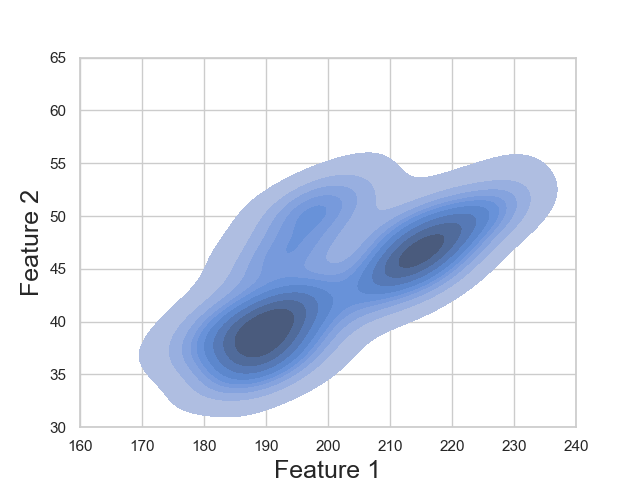
\includegraphics[width=.6\textwidth]{img/viz/kde2d_1}
\end{frame}


\begin{frame}{2D distribution}
  \centering
  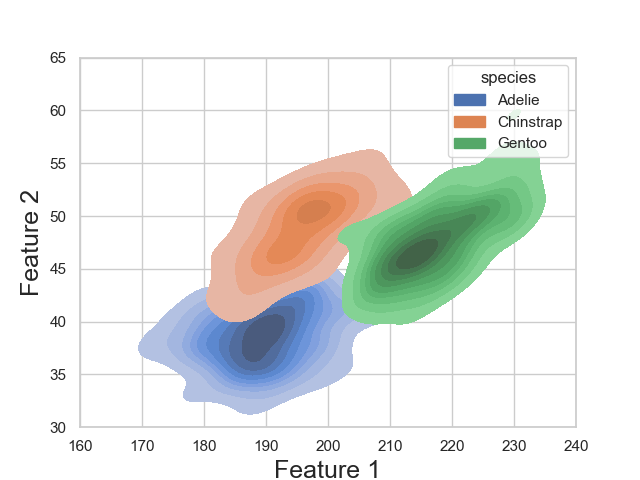
\includegraphics[width=.6\textwidth]{img/viz/kde2d_2}
\end{frame}

\begin{frame}{3D distribution}
  \centering
  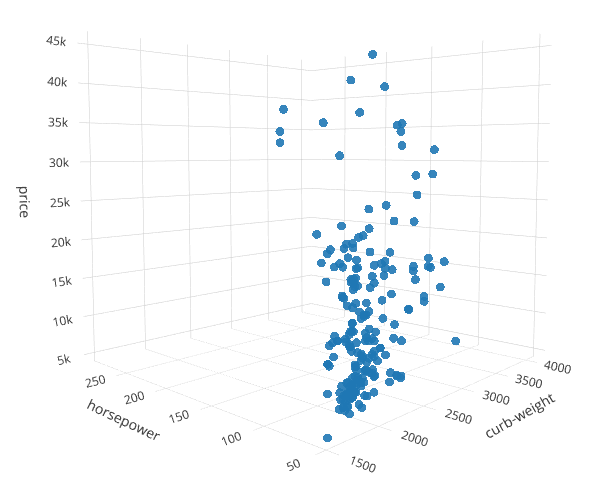
\includegraphics[width=.6\textwidth]{img/viz/scatter_3d}

  Source: \href{https://medium.com/@prasadostwal/multi-dimension-plots-in-python-from-2d-to-6d-9a2bf7b8cc74}{medium.com}
\end{frame}

% 4D to 6D scatter
\begin{frame}{High-dimensional: scatter plot}

  How to visualize points in a higher dimension than 3?

  \begin{block}{Key points}
    \begin{itemize}
      \item Add \textcolor{red}{colors} w.r.t. the values of an additional variable
      \item Add different \textcolor{red}{sizes} proportional to the values of an additional variable
      \item Add differnet \textcolor{red}{shapes} to the points
    \end{itemize}
  \end{block}

\end{frame}


\begin{frame}{High-dimensional: 4D scatter plot}
\begin{center}
  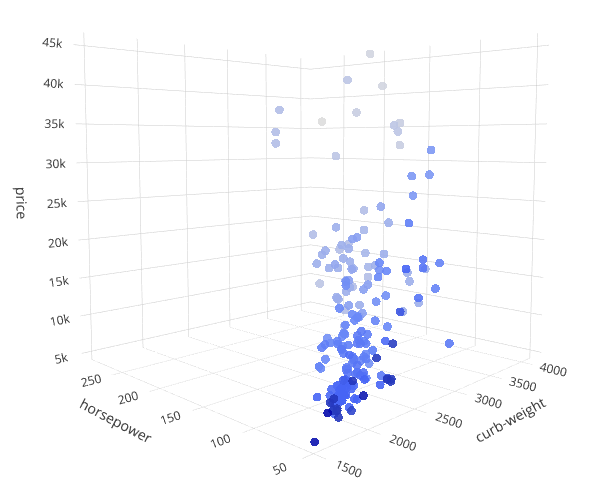
\includegraphics[width=.6\textwidth]{img/viz/scatter_4d}
  \begin{itemize}
    \item Add colors w.r.t. the values of an additional variable
  \end{itemize}
\end{center}

Source: \href{https://medium.com/@prasadostwal/multi-dimension-plots-in-python-from-2d-to-6d-9a2bf7b8cc74}{medium.com}
\end{frame}


\begin{frame}{High-dimensional: 5D scatter plot}
\begin{center}
  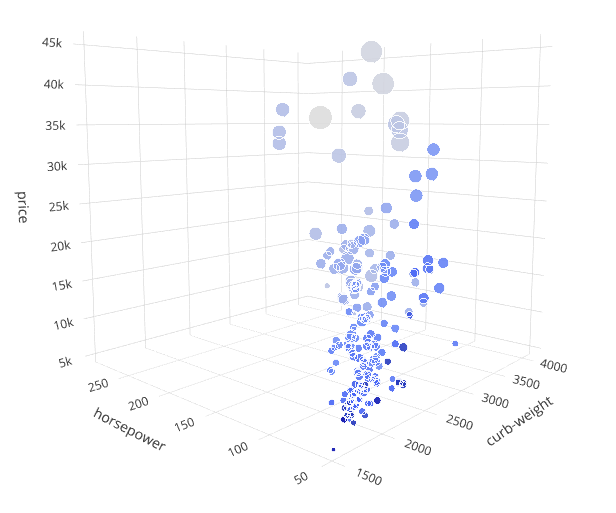
\includegraphics[width=.6\textwidth]{img/viz/scatter_5d}
  \begin{itemize}
    \item Add different sizes w.r.t. to the values of an additional variable
  \end{itemize}
\end{center}

Source: \href{https://medium.com/@prasadostwal/multi-dimension-plots-in-python-from-2d-to-6d-9a2bf7b8cc74}{medium.com}
\end{frame}


\begin{frame}{High-dimensional: 6D scatter plot}
\begin{center}
  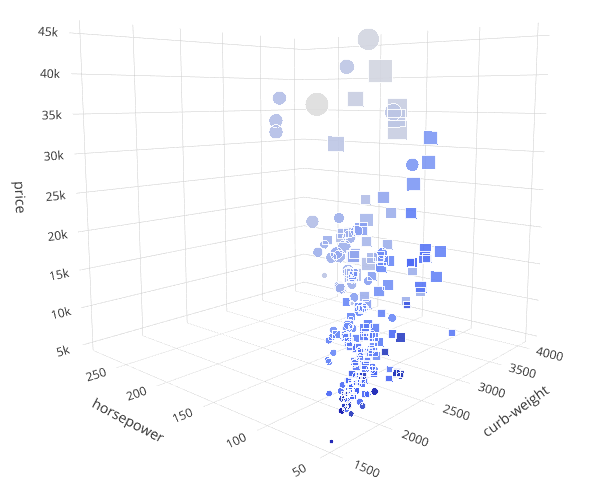
\includegraphics[width=.6\textwidth]{img/viz/scatter_6d}
  \begin{itemize}
    \item Add different shapes to the points
  \end{itemize}
\end{center}

Source: \href{https://medium.com/@prasadostwal/multi-dimension-plots-in-python-from-2d-to-6d-9a2bf7b8cc74}{medium.com}
\end{frame}


\begin{frame}{High-dimensional: radar plot}
  \centering
  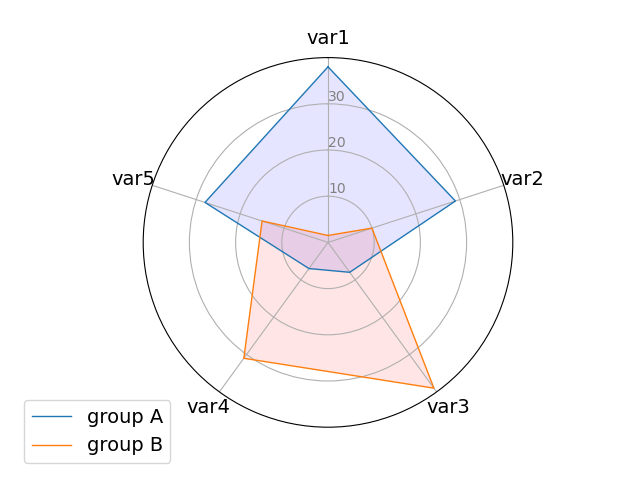
\includegraphics[width=\textwidth]{img/viz/radar}
\end{frame}


\begin{frame}{Maps}
  \centering
  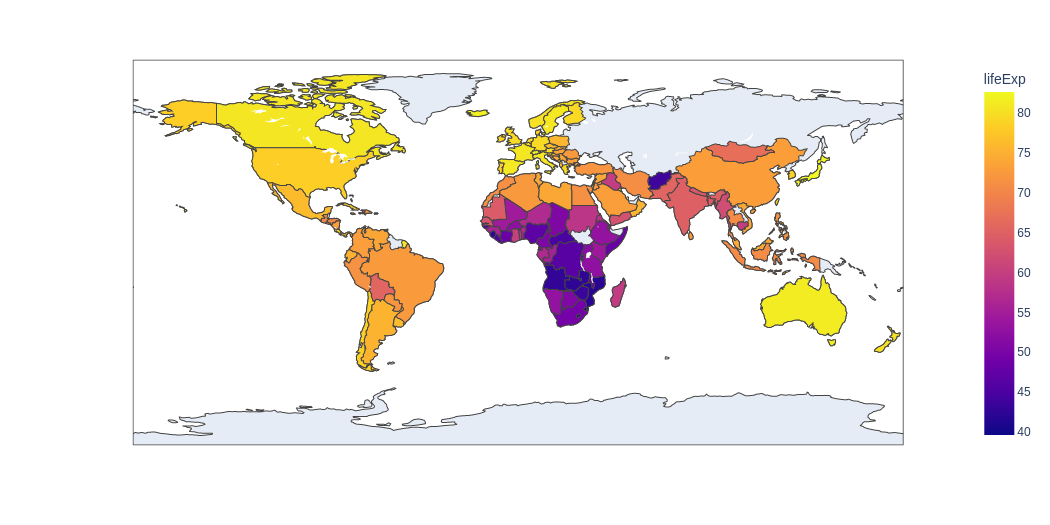
\includegraphics[width=.9\textwidth]{img/viz/map}
\end{frame}


\begin{frame}{Maps}
  \centering
  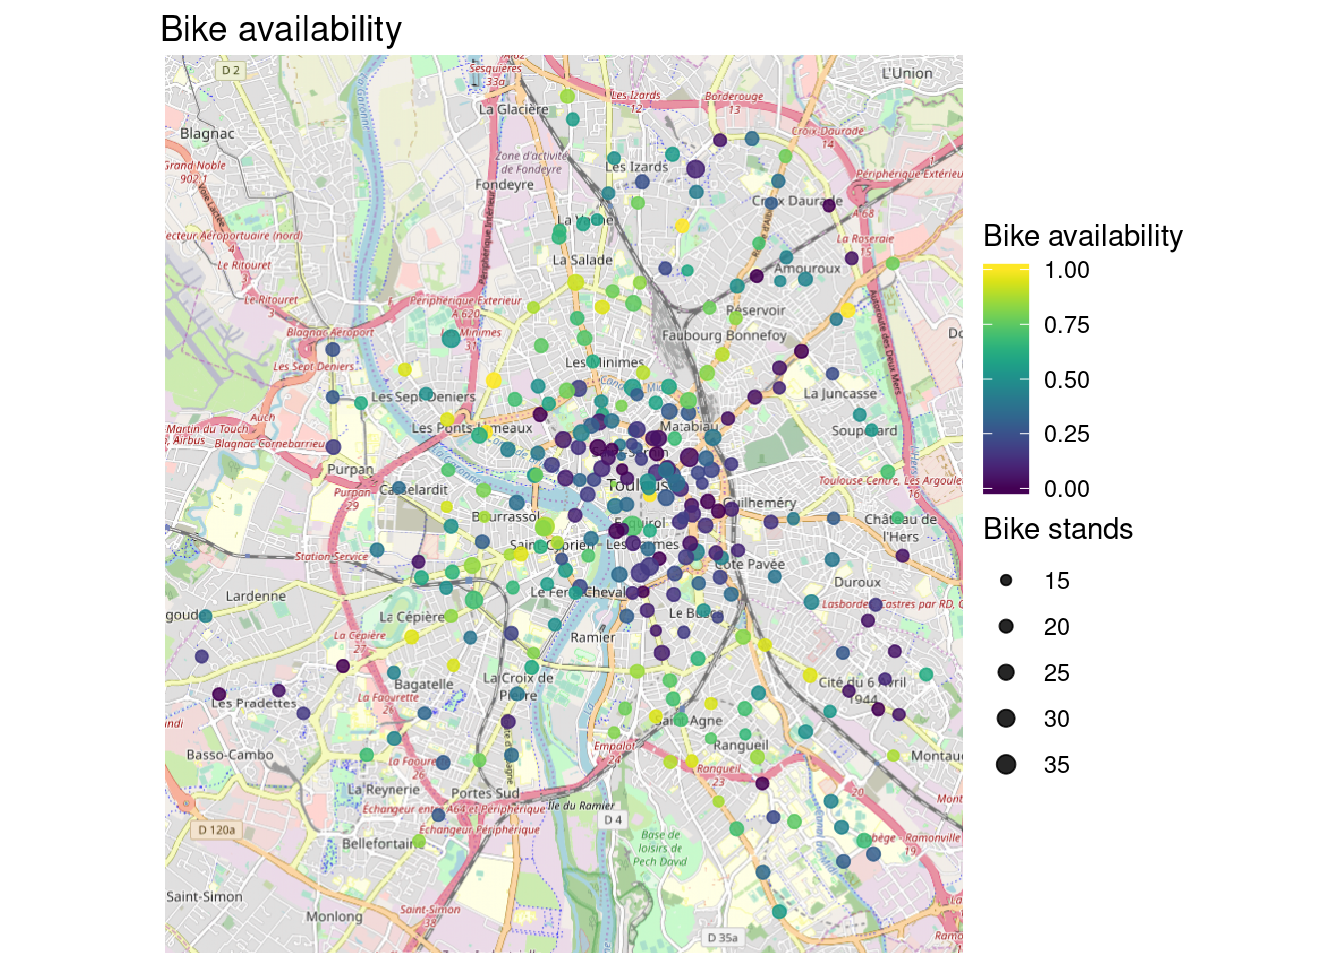
\includegraphics[width=.8\textwidth]{img/viz/map2}
\end{frame}

\begin{frame}{Networks}
  \centering
  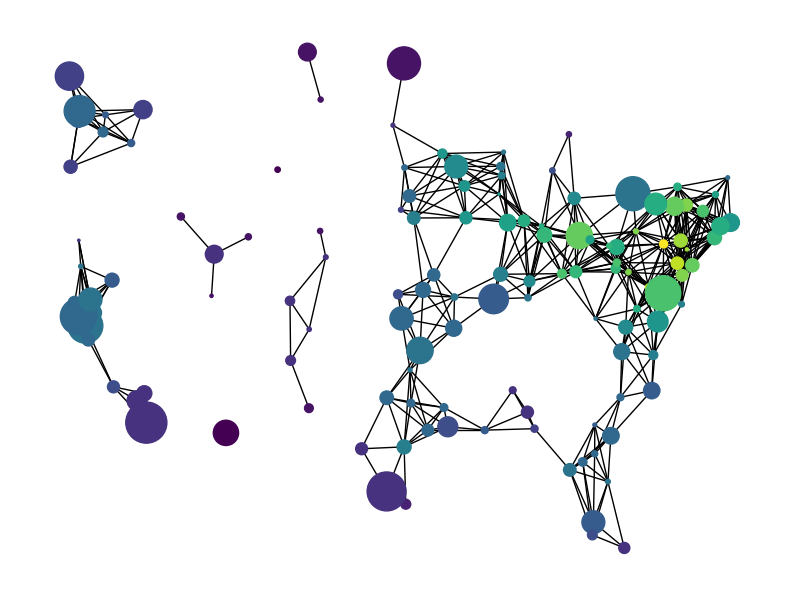
\includegraphics[width=.8\textwidth]{img/viz/network}
\end{frame}



\section{En résumé}

\begin{frame}{En résumé}
  \begin{block}{Le data mining c'est}
    \begin{itemize}
      \item Le fait de tirer de l'information de données.
      \item un moyen de prendre des décision
    \end{itemize}
  \end{block}

  \begin{block}{Comment ?}
    \begin{itemize}
      \item Analyses statistiques
      \item Visualisation de données
      \item Apprentissage automatique
    \end{itemize}
  \end{block}

\end{frame}



\begin{frame}

  \begin{center}
    {\Large Merci pour votre attention}

    \bigskip

    
\includegraphics[height=1.5cm]{img/logo_scai.png}
  \end{center}

\end{frame}

\end{document}
 